% =============================================================================
% EAI Endorsed Transactions -- Journal Submission Draft
% "Reward Contrast, Not Algorithm Labels" -- TinkerRL Audit
% Format: EAI-compliant preamble (single-column, Vancouver references).
% Drop-in replace \documentclass with the official eai_temp.cls when acquired.
% =============================================================================

\documentclass[a4paper,10pt]{article}

% --- Geometry matching EAI Endorsed Transactions A4 layout ---------------------
\usepackage[a4paper,top=2.2cm,bottom=2.4cm,left=2.0cm,right=2.0cm,headsep=0.6cm]{geometry}

% --- Font / encoding -----------------------------------------------------------
\usepackage[utf8]{inputenc}
\usepackage[T1]{fontenc}
\usepackage{mathptmx}      % Times-like (EAI uses a serif body font)
\usepackage{helvet}        % Arial/Helvetica for headings
\usepackage{courier}
\renewcommand{\familydefault}{\rmdefault}

% --- Bibliography: Vancouver (required by EAI) ---------------------------------
\usepackage[numbers,sort&compress,super]{natbib}
\bibliographystyle{vancouver}

% --- Standard math / graphics / tables -----------------------------------------
\usepackage{amsmath,amssymb,amsfonts}
\usepackage{nicefrac}
\usepackage{microtype}
\usepackage{xcolor}
\usepackage{graphicx}
\usepackage{subcaption}
\usepackage{booktabs}
\usepackage{multirow}
\usepackage{enumitem}
\usepackage{algorithm}
\usepackage{algorithmic}
\usepackage{url}
\usepackage[hidelinks]{hyperref}
\usepackage{tikz}
\usetikzlibrary{positioning,fit,arrows.meta,backgrounds,calc,shadows,shapes.geometric,shapes.misc,decorations.pathreplacing}

\graphicspath{{.}{figures/}{figures/v2/}{tikz/}}

% --- EAI header/footer rules ---------------------------------------------------
\usepackage{fancyhdr}
\pagestyle{fancy}
\fancyhf{}
\fancyhead[L]{\small EAI Endorsed Transactions}
\fancyhead[R]{\small Preprint Draft}
\fancyfoot[C]{\thepage}
\renewcommand{\headrulewidth}{0.4pt}

% --- Title spacing akin to EAI journal title block ----------------------------
\usepackage{titling}
\setlength{\droptitle}{-1.0cm}

% --- Keywords environment (EAI submission requires 3–8 keywords) --------------
\providecommand{\keywords}[1]{\par\noindent\textbf{Keywords:} #1}

% --- Custom short commands used throughout the manuscript ---------------------
\newcommand{\tinker}{\textsc{Tinker}}
\newcommand{\atropos}{\textsc{Atropos}}
\newcommand{\grpo}{\textsc{Grpo}}
\newcommand{\ours}{\textsc{TinkerRL Audit}}

% --- Shim commands formerly provided by neurips_2026.sty ----------------------
% The NeurIPS checklist is removed for the EAI format; answer macros shimmed
% only so any stray reference still compiles.
\newcommand{\answerYes}[1][]{\textcolor{black}{[Yes] #1}}
\newcommand{\answerNo}[1][]{\textcolor{black}{[No] #1}}
\newcommand{\answerNA}[1][]{\textcolor{black}{[N/A] #1}}
\newcommand{\answerTODO}[1][]{\textcolor{black}{[TODO] #1}}
\newcommand{\answerPartial}[1][]{\textcolor{black}{[Partial] #1}}
\newenvironment{ack}{\section*{Acknowledgements}}{}

% --- Title ---------------------------------------------------------------------
\title{\fontsize{16pt}{18pt}\selectfont\bfseries
Reward Contrast, Not Algorithm Labels:\\
A Diagnostic Audit of Critic-Free Group-Relative RL for LLMs}

\author{%
  Arvind C R$^{1,\ast}$, Sandhya Jeyaraj$^{1,\ast}$, Madhu Kumara L$^{1}$,
  Mohammad Rafi$^{1}$, Dhruva N Murthy$^{1}$, Arumugam K$^{1}$,\\
  Anwesh Reddy Paduri$^{2}$, Narayana Darapaneni$^{3}$\\[4pt]
  \small
  $^{1}$PES University, Bengaluru, India \\
  $^{2}$Great Learning / PES University, India \\
  $^{3}$Northwestern University / Great Learning, USA \\
  $^{\ast}$Equal contribution.\\
  \texttt{\{arvindcr4, sandhya.jeyaraj2014, madhukumara1993, gmd.rafi.2024,
  dhruva.n.murthy, chettyarumugam\}@gmail.com}\\
  \texttt{anwesh@greatlearning.in}, \texttt{narayana.darapaneni@northwestern.edu}
}
\date{}

\begin{document}
% Removed global badness/overflow suppression (\sloppy, \hbadness=10000,
% \vbadness=10000, \hfuzz=2pt) that masked layout issues. Individual
% overfull boxes are now fixed locally where they occur.

\maketitle
\thispagestyle{fancy}

% =============================================================================
% Abstract + EAI required keywords
% =============================================================================
% EAI-compliant structured abstract (PubMed style, <=1000 chars).
\begin{abstract}
\noindent\textbf{Background:} Group-relative RL for LLMs (PPO, GRPO, DPO) is
typically judged at the algorithm-label level, ignoring the
model--reward--sampler--stack combination behind each observation.
\textbf{Methods:} We audit the stack with two triage diagnostics:
Zero-Variance Fraction (ZVF, the share of prompts where all $G$ samples
receive identical reward) and Gradient Utilization $=1-$ZVF.
\textbf{Results:} A fixed first-five-step rule (ZVF$\geq$80\%, reward$\leq$5\%)
triages collapsed runs in a 22-run set with only 2 positive cases
(power-bounded). Online reward and capability diverge: Qwen3-8B gains only
82.0$\to$83.3\% on held-out GSM8K; the two real cross-stack runs (Tinker,
TRL) differ $\approx$17$\times$ in last-10 reward; verl/OpenRLHF are
dry-run placeholders.
\textbf{Conclusions:} The algorithm label alone is an under-specified
experimental treatment; usable signal must be verified per stack.
Code released.
\end{abstract}


\keywords{reinforcement learning, RLVR, GRPO, PPO, large language models,
reward contrast, diagnostic audit, reproducibility}

% =============================================================================
% Body (content unchanged from main.tex)
% =============================================================================
% =============================================================================
% Introduction -- evidence-hierarchy rewrite
% Drop-in include: % =============================================================================
% Introduction -- evidence-hierarchy rewrite
% Drop-in include: % =============================================================================
% Introduction -- evidence-hierarchy rewrite
% Drop-in include: \input{sections/intro}
% =============================================================================
\section{Introduction}
\label{sec:intro}

This paper separates three kinds of evidence before making any claim about
reinforcement-learning post-training.  Held-out evaluations are the only basis
we use for capability claims.  Online rewards are evidence about optimization
inside a particular reward environment.  Proxy rewards, partial harnesses, and
stack-specific comparisons are treated as hypotheses or diagnostics unless they
are paired with matched held-out evaluation.  This hierarchy is necessary
because PPO~\citep{schulman2017proximal}, GRPO~\citep{shao2024deepseekmath},
and DPO~\citep{rafailov2024direct} are often discussed as algorithm-level
interventions, while LLM post-training outcomes also depend on base model,
instruction tuning, reward parser, group construction, sampler, backend, LoRA
configuration, checkpoint selection, and evaluation harness.  The resulting
identification problem is the LLM post-training analogue of the reproducibility
concerns identified by Henderson et al.~\citep{henderson2018deep} for deep RL.

On the strongest evidence tier, this paper does \emph{not} show that GRPO
broadly improves reasoning.  The clean held-out capability check is a GSM8K
200-example slice that was not used during training, and it improves only from
$82.0\%$ to $83.3\%$ ($p=0.26$).  We therefore do not claim a significant
held-out math effect.  This negative result determines the scope of the rest of
the paper: training reward curves and proxy environments may explain when a
post-training loop has signal, but they do not establish general reasoning or
tool-use capability.

Within that scope, \ours{} is a systems audit of a group-relative RL runner
rather than an algorithm leaderboard.  The corpus contains 79 runs across
structured tool-call emission, GSM8K, MATH-style tasks, HumanEval-style binary
verification, small and frontier-scale model families, and several training
backends.  The runner is inspired by GRPO, but it is not a faithful reproduction
of canonical GRPO: it keeps group-normalized advantages and a critic-free
structure, but it does not implement the PPO probability ratio and clip of
\citet{schulman2017proximal}, does not keep a frozen reference policy for KL
regularization, performs one optimizer step per rollout batch, and does not use
a completion-only token mask.  A P1-A diagnostic on Qwen3.5-4B measures
$61.6\%$--$89.6\%$ of the full-sequence loss magnitude as coming from prompt
tokens rather than completion tokens.  Claims below therefore concern this
runner and its reward environments, not a universal property of canonical GRPO.

The paper's main positive claim sits one tier below held-out capability: the
runner behaves as a reward-contrast amplifier.  In a critic-free group-relative
update, a prompt is useful only when the sampled group contains distinguishable
reward outcomes.  Under binary or verifier-like rewards, if the current policy
succeeds on prompt $x$ with probability $p_x$ and the group size is $G$, the
probability of obtaining a mixed, gradient-carrying group is approximated by
\[
P(\text{usable}) \approx \frac{1}{N}\sum_x \left[1 - (1-p_x)^G - p_x^G\right].
\]
This mechanism explains why warm-starts, group size, reward density, and task
difficulty matter more than task labels.  The familiar $p_x > 1/G$ rule is only
an expected-one-success heuristic; it is not a threshold theorem for learning.

Zero-Variance Fraction (ZVF) and Gradient Utilization (GU) operationalize that
mechanism as diagnostics, not as capability metrics.  ZVF is the fraction of
sampled groups whose rewards are all identical, and GU is its complement.  High
ZVF with low reward indicates cold-start collapse because all completions are
unrewarded and the group-relative advantage is flat.  High ZVF with high reward
indicates saturation because the reward environment is already mostly solved.
Low ZVF indicates that the current policy still samples both successes and
failures, giving the update within-group contrast.  In a 22-run de-duplicated
validation set, a fixed first-five-step rule catches both collapsed runs with no
false positives, but only two positive failures are observed and continuous ZVF
ranking is weak.  The defensible claim is therefore triage: ZVF/GU can support
early decisions to stop, warm-start, densify reward, adjust task difficulty, or
change group size.

Several reward environments in the audit remain lower-tier evidence because
they measure proxies rather than end-to-end capability.  The tool-use reward
scores JSON well-formedness, tool-name selection, and argument-key presence
without executing tools.  The HumanEval-style sandbox executes completions in a
restricted environment with Python built-ins removed, rejecting some legitimate
programs that use functions such as \texttt{len}, \texttt{range}, or
\texttt{sum}.  The MATH reward combines \texttt{\textbackslash boxed\{\}}
format credit with final-answer matching.  In addition, the MATH-500 and
HumanEval prompt pools used inside the training loop are loaded from the
\texttt{test} splits of their respective datasets, so they function here as
reward-environment probes rather than held-out generalization tests.  Positive
rows in these settings are useful evidence about reward dynamics and verifier
interaction, not proof of broad tool use, coding, or mathematical reasoning.

Algorithm comparisons are also lower-tier unless the full stack is fixed or
modeled.  The PPO/GRPO/DPO label alone is not an experimental treatment.  Our
Qwen PPO/GRPO comparison is artifact-sensitive: the source-of-truth ledger
records PPO at 0.225 last-10 reward, while a statistical summary records 0.350.
The Llama-3.1-8B-Instruct comparison favors PPO over the group-relative runner.
These observations should not be converted into a universal PPO-versus-GRPO
ranking.  They instead motivate stack-conditioned reporting of model family,
backend, reward implementation, rollout sampler, optimizer and KL handling,
LoRA target modules, checkpoint-selection rule, and evaluation slice.

\begin{table}[t]
\centering
\caption{Claim--evidence--verdict hierarchy used throughout the paper.}
\label{tab:claim_evidence_verdict}
\small
\begin{tabular}{@{}p{0.27\linewidth}p{0.18\linewidth}p{0.33\linewidth}p{0.16\linewidth}@{}}
\toprule
\textbf{Claim} & \textbf{Status} & \textbf{Headline evidence} & \textbf{Verdict}\\
\midrule
C1: The GRPO-style runner is a reward-contrast amplifier. & Most original contribution &
Mixed-group probability, early-run ZVF/GU, measured base-hit-rate audits, and collapse/saturation cases. &
Signal exists only when sampled groups contain reward diversity.\\
C2: PPO/GRPO/DPO labels are under-specified treatments. & Methodological contribution &
Qwen artifact sensitivity, the Llama PPO-favored row, and backend/model/reward/parser confounding. &
No universal algorithm ranking.\\
C3: Training reward does not equal capability. & Central negative result &
Held-out GSM8K $82.0\%\!\to\!83.3\%$ ($p=0.26$); tool-use rewards are
proxy/schema rewards; HumanEval/MATH harnesses are limited. &
Training reward supports dynamics claims only.\\
\bottomrule
\end{tabular}
\end{table}

The contributions follow this hierarchy.  First, we report the negative
held-out GSM8K result as the boundary on capability claims.  Second, we give a
mechanistic account of when a group-relative runner has a learning signal via
mixed-reward sampling probability.  Third, we introduce ZVF/GU as early-run
triage diagnostics for collapse and saturation.  Fourth, we document how proxy
rewards, parser choices, and sandbox constraints affect the interpretation of
training reward.  Fifth, we provide a source-of-truth ledger and reporting
recommendations showing why PPO, GRPO, and DPO comparisons require full-stack
specification.  We release the code, run logs, and checkpoints at
\url{https://anonymous.4open.science/r/tinker-rl-lab}.

% =============================================================================
\section{Introduction}
\label{sec:intro}

This paper separates three kinds of evidence before making any claim about
reinforcement-learning post-training.  Held-out evaluations are the only basis
we use for capability claims.  Online rewards are evidence about optimization
inside a particular reward environment.  Proxy rewards, partial harnesses, and
stack-specific comparisons are treated as hypotheses or diagnostics unless they
are paired with matched held-out evaluation.  This hierarchy is necessary
because PPO~\citep{schulman2017proximal}, GRPO~\citep{shao2024deepseekmath},
and DPO~\citep{rafailov2024direct} are often discussed as algorithm-level
interventions, while LLM post-training outcomes also depend on base model,
instruction tuning, reward parser, group construction, sampler, backend, LoRA
configuration, checkpoint selection, and evaluation harness.  The resulting
identification problem is the LLM post-training analogue of the reproducibility
concerns identified by Henderson et al.~\citep{henderson2018deep} for deep RL.

On the strongest evidence tier, this paper does \emph{not} show that GRPO
broadly improves reasoning.  The clean held-out capability check is a GSM8K
200-example slice that was not used during training, and it improves only from
$82.0\%$ to $83.3\%$ ($p=0.26$).  We therefore do not claim a significant
held-out math effect.  This negative result determines the scope of the rest of
the paper: training reward curves and proxy environments may explain when a
post-training loop has signal, but they do not establish general reasoning or
tool-use capability.

Within that scope, \ours{} is a systems audit of a group-relative RL runner
rather than an algorithm leaderboard.  The corpus contains 79 runs across
structured tool-call emission, GSM8K, MATH-style tasks, HumanEval-style binary
verification, small and frontier-scale model families, and several training
backends.  The runner is inspired by GRPO, but it is not a faithful reproduction
of canonical GRPO: it keeps group-normalized advantages and a critic-free
structure, but it does not implement the PPO probability ratio and clip of
\citet{schulman2017proximal}, does not keep a frozen reference policy for KL
regularization, performs one optimizer step per rollout batch, and does not use
a completion-only token mask.  A P1-A diagnostic on Qwen3.5-4B measures
$61.6\%$--$89.6\%$ of the full-sequence loss magnitude as coming from prompt
tokens rather than completion tokens.  Claims below therefore concern this
runner and its reward environments, not a universal property of canonical GRPO.

The paper's main positive claim sits one tier below held-out capability: the
runner behaves as a reward-contrast amplifier.  In a critic-free group-relative
update, a prompt is useful only when the sampled group contains distinguishable
reward outcomes.  Under binary or verifier-like rewards, if the current policy
succeeds on prompt $x$ with probability $p_x$ and the group size is $G$, the
probability of obtaining a mixed, gradient-carrying group is approximated by
\[
P(\text{usable}) \approx \frac{1}{N}\sum_x \left[1 - (1-p_x)^G - p_x^G\right].
\]
This mechanism explains why warm-starts, group size, reward density, and task
difficulty matter more than task labels.  The familiar $p_x > 1/G$ rule is only
an expected-one-success heuristic; it is not a threshold theorem for learning.

Zero-Variance Fraction (ZVF) and Gradient Utilization (GU) operationalize that
mechanism as diagnostics, not as capability metrics.  ZVF is the fraction of
sampled groups whose rewards are all identical, and GU is its complement.  High
ZVF with low reward indicates cold-start collapse because all completions are
unrewarded and the group-relative advantage is flat.  High ZVF with high reward
indicates saturation because the reward environment is already mostly solved.
Low ZVF indicates that the current policy still samples both successes and
failures, giving the update within-group contrast.  In a 22-run de-duplicated
validation set, a fixed first-five-step rule catches both collapsed runs with no
false positives, but only two positive failures are observed and continuous ZVF
ranking is weak.  The defensible claim is therefore triage: ZVF/GU can support
early decisions to stop, warm-start, densify reward, adjust task difficulty, or
change group size.

Several reward environments in the audit remain lower-tier evidence because
they measure proxies rather than end-to-end capability.  The tool-use reward
scores JSON well-formedness, tool-name selection, and argument-key presence
without executing tools.  The HumanEval-style sandbox executes completions in a
restricted environment with Python built-ins removed, rejecting some legitimate
programs that use functions such as \texttt{len}, \texttt{range}, or
\texttt{sum}.  The MATH reward combines \texttt{\textbackslash boxed\{\}}
format credit with final-answer matching.  In addition, the MATH-500 and
HumanEval prompt pools used inside the training loop are loaded from the
\texttt{test} splits of their respective datasets, so they function here as
reward-environment probes rather than held-out generalization tests.  Positive
rows in these settings are useful evidence about reward dynamics and verifier
interaction, not proof of broad tool use, coding, or mathematical reasoning.

Algorithm comparisons are also lower-tier unless the full stack is fixed or
modeled.  The PPO/GRPO/DPO label alone is not an experimental treatment.  Our
Qwen PPO/GRPO comparison is artifact-sensitive: the source-of-truth ledger
records PPO at 0.225 last-10 reward, while a statistical summary records 0.350.
The Llama-3.1-8B-Instruct comparison favors PPO over the group-relative runner.
These observations should not be converted into a universal PPO-versus-GRPO
ranking.  They instead motivate stack-conditioned reporting of model family,
backend, reward implementation, rollout sampler, optimizer and KL handling,
LoRA target modules, checkpoint-selection rule, and evaluation slice.

\begin{table}[t]
\centering
\caption{Claim--evidence--verdict hierarchy used throughout the paper.}
\label{tab:claim_evidence_verdict}
\small
\begin{tabular}{@{}p{0.27\linewidth}p{0.18\linewidth}p{0.33\linewidth}p{0.16\linewidth}@{}}
\toprule
\textbf{Claim} & \textbf{Status} & \textbf{Headline evidence} & \textbf{Verdict}\\
\midrule
C1: The GRPO-style runner is a reward-contrast amplifier. & Most original contribution &
Mixed-group probability, early-run ZVF/GU, measured base-hit-rate audits, and collapse/saturation cases. &
Signal exists only when sampled groups contain reward diversity.\\
C2: PPO/GRPO/DPO labels are under-specified treatments. & Methodological contribution &
Qwen artifact sensitivity, the Llama PPO-favored row, and backend/model/reward/parser confounding. &
No universal algorithm ranking.\\
C3: Training reward does not equal capability. & Central negative result &
Held-out GSM8K $82.0\%\!\to\!83.3\%$ ($p=0.26$); tool-use rewards are
proxy/schema rewards; HumanEval/MATH harnesses are limited. &
Training reward supports dynamics claims only.\\
\bottomrule
\end{tabular}
\end{table}

The contributions follow this hierarchy.  First, we report the negative
held-out GSM8K result as the boundary on capability claims.  Second, we give a
mechanistic account of when a group-relative runner has a learning signal via
mixed-reward sampling probability.  Third, we introduce ZVF/GU as early-run
triage diagnostics for collapse and saturation.  Fourth, we document how proxy
rewards, parser choices, and sandbox constraints affect the interpretation of
training reward.  Fifth, we provide a source-of-truth ledger and reporting
recommendations showing why PPO, GRPO, and DPO comparisons require full-stack
specification.  We release the code, run logs, and checkpoints at
\url{https://anonymous.4open.science/r/tinker-rl-lab}.

% =============================================================================
\section{Introduction}
\label{sec:intro}

This paper separates three kinds of evidence before making any claim about
reinforcement-learning post-training.  Held-out evaluations are the only basis
we use for capability claims.  Online rewards are evidence about optimization
inside a particular reward environment.  Proxy rewards, partial harnesses, and
stack-specific comparisons are treated as hypotheses or diagnostics unless they
are paired with matched held-out evaluation.  This hierarchy is necessary
because PPO~\citep{schulman2017proximal}, GRPO~\citep{shao2024deepseekmath},
and DPO~\citep{rafailov2024direct} are often discussed as algorithm-level
interventions, while LLM post-training outcomes also depend on base model,
instruction tuning, reward parser, group construction, sampler, backend, LoRA
configuration, checkpoint selection, and evaluation harness.  The resulting
identification problem is the LLM post-training analogue of the reproducibility
concerns identified by Henderson et al.~\citep{henderson2018deep} for deep RL.

On the strongest evidence tier, this paper does \emph{not} show that GRPO
broadly improves reasoning.  The clean held-out capability check is a GSM8K
200-example slice that was not used during training, and it improves only from
$82.0\%$ to $83.3\%$ ($p=0.26$).  We therefore do not claim a significant
held-out math effect.  This negative result determines the scope of the rest of
the paper: training reward curves and proxy environments may explain when a
post-training loop has signal, but they do not establish general reasoning or
tool-use capability.

Within that scope, \ours{} is a systems audit of a group-relative RL runner
rather than an algorithm leaderboard.  The corpus contains 79 runs across
structured tool-call emission, GSM8K, MATH-style tasks, HumanEval-style binary
verification, small and frontier-scale model families, and several training
backends.  The runner is inspired by GRPO, but it is not a faithful reproduction
of canonical GRPO: it keeps group-normalized advantages and a critic-free
structure, but it does not implement the PPO probability ratio and clip of
\citet{schulman2017proximal}, does not keep a frozen reference policy for KL
regularization, performs one optimizer step per rollout batch, and does not use
a completion-only token mask.  A P1-A diagnostic on Qwen3.5-4B measures
$61.6\%$--$89.6\%$ of the full-sequence loss magnitude as coming from prompt
tokens rather than completion tokens.  Claims below therefore concern this
runner and its reward environments, not a universal property of canonical GRPO.

The paper's main positive claim sits one tier below held-out capability: the
runner behaves as a reward-contrast amplifier.  In a critic-free group-relative
update, a prompt is useful only when the sampled group contains distinguishable
reward outcomes.  Under binary or verifier-like rewards, if the current policy
succeeds on prompt $x$ with probability $p_x$ and the group size is $G$, the
probability of obtaining a mixed, gradient-carrying group is approximated by
\[
P(\text{usable}) \approx \frac{1}{N}\sum_x \left[1 - (1-p_x)^G - p_x^G\right].
\]
This mechanism explains why warm-starts, group size, reward density, and task
difficulty matter more than task labels.  The familiar $p_x > 1/G$ rule is only
an expected-one-success heuristic; it is not a threshold theorem for learning.

Zero-Variance Fraction (ZVF) and Gradient Utilization (GU) operationalize that
mechanism as diagnostics, not as capability metrics.  ZVF is the fraction of
sampled groups whose rewards are all identical, and GU is its complement.  High
ZVF with low reward indicates cold-start collapse because all completions are
unrewarded and the group-relative advantage is flat.  High ZVF with high reward
indicates saturation because the reward environment is already mostly solved.
Low ZVF indicates that the current policy still samples both successes and
failures, giving the update within-group contrast.  In a 22-run de-duplicated
validation set, a fixed first-five-step rule catches both collapsed runs with no
false positives, but only two positive failures are observed and continuous ZVF
ranking is weak.  The defensible claim is therefore triage: ZVF/GU can support
early decisions to stop, warm-start, densify reward, adjust task difficulty, or
change group size.

Several reward environments in the audit remain lower-tier evidence because
they measure proxies rather than end-to-end capability.  The tool-use reward
scores JSON well-formedness, tool-name selection, and argument-key presence
without executing tools.  The HumanEval-style sandbox executes completions in a
restricted environment with Python built-ins removed, rejecting some legitimate
programs that use functions such as \texttt{len}, \texttt{range}, or
\texttt{sum}.  The MATH reward combines \texttt{\textbackslash boxed\{\}}
format credit with final-answer matching.  In addition, the MATH-500 and
HumanEval prompt pools used inside the training loop are loaded from the
\texttt{test} splits of their respective datasets, so they function here as
reward-environment probes rather than held-out generalization tests.  Positive
rows in these settings are useful evidence about reward dynamics and verifier
interaction, not proof of broad tool use, coding, or mathematical reasoning.

Algorithm comparisons are also lower-tier unless the full stack is fixed or
modeled.  The PPO/GRPO/DPO label alone is not an experimental treatment.  Our
Qwen PPO/GRPO comparison is artifact-sensitive: the source-of-truth ledger
records PPO at 0.225 last-10 reward, while a statistical summary records 0.350.
The Llama-3.1-8B-Instruct comparison favors PPO over the group-relative runner.
These observations should not be converted into a universal PPO-versus-GRPO
ranking.  They instead motivate stack-conditioned reporting of model family,
backend, reward implementation, rollout sampler, optimizer and KL handling,
LoRA target modules, checkpoint-selection rule, and evaluation slice.

\begin{table}[t]
\centering
\caption{Claim--evidence--verdict hierarchy used throughout the paper.}
\label{tab:claim_evidence_verdict}
\small
\begin{tabular}{@{}p{0.27\linewidth}p{0.18\linewidth}p{0.33\linewidth}p{0.16\linewidth}@{}}
\toprule
\textbf{Claim} & \textbf{Status} & \textbf{Headline evidence} & \textbf{Verdict}\\
\midrule
C1: The GRPO-style runner is a reward-contrast amplifier. & Most original contribution &
Mixed-group probability, early-run ZVF/GU, measured base-hit-rate audits, and collapse/saturation cases. &
Signal exists only when sampled groups contain reward diversity.\\
C2: PPO/GRPO/DPO labels are under-specified treatments. & Methodological contribution &
Qwen artifact sensitivity, the Llama PPO-favored row, and backend/model/reward/parser confounding. &
No universal algorithm ranking.\\
C3: Training reward does not equal capability. & Central negative result &
Held-out GSM8K $82.0\%\!\to\!83.3\%$ ($p=0.26$); tool-use rewards are
proxy/schema rewards; HumanEval/MATH harnesses are limited. &
Training reward supports dynamics claims only.\\
\bottomrule
\end{tabular}
\end{table}

The contributions follow this hierarchy.  First, we report the negative
held-out GSM8K result as the boundary on capability claims.  Second, we give a
mechanistic account of when a group-relative runner has a learning signal via
mixed-reward sampling probability.  Third, we introduce ZVF/GU as early-run
triage diagnostics for collapse and saturation.  Fourth, we document how proxy
rewards, parser choices, and sandbox constraints affect the interpretation of
training reward.  Fifth, we provide a source-of-truth ledger and reporting
recommendations showing why PPO, GRPO, and DPO comparisons require full-stack
specification.  We release the code, run logs, and checkpoints at
\url{https://anonymous.4open.science/r/tinker-rl-lab}.

% =============================================================================
% Related Work v2 --- expanded related work for NeurIPS 2026 submission
% Replaces the Related Work section in paper/main.tex (sec:related).
% Grouped into five themes:
%   (1) RL algorithms for LLMs
%   (2) Reasoning RL (and process reward models)
%   (3) Tool-use RL
%   (4) Scale and reward-trajectory evidence for RL post-training
%   (5) Frameworks, evaluation harnesses, and reproducibility
% Every paragraph references entries defined in paper/references.bib.
% =============================================================================

\section{Related Work}
\label{sec:related}

\ours{} is not an optimizer paper in the style of DeepSeekMath, nor a
new zero-variance optimizer or prompt-selection rule in the style of RL-ZVP or
Online Difficulty Filtering.  It is a systems-oriented empirical audit of when
group-relative LLM post-training has a usable reward-contrast signal and when
its rewards become misleading evidence.  We therefore position the work along
five axes: policy-gradient \emph{algorithms} for language models, RL for
\emph{reasoning} (including process reward models and spurious-reward studies),
RL for \emph{tool use} and agentic behaviour, descriptive scale and
reward-trajectory studies for RL post-training, and the \emph{frameworks},
\emph{evaluation harnesses}, and reproducibility practices that instantiate
these algorithms.  The recurring
claim is that an algorithm label is not the full treatment: the model family,
reward parser, sampler, backend, mask, checkpoint rule, and evaluation split all
condition what a reported RL gain means.

% -----------------------------------------------------------------------------
\subsection{RL Algorithms for Large Language Models}
\label{sec:related:algos}

Proximal Policy Optimization (PPO)~\cite{schulman2017proximal} is the workhorse
algorithm behind InstructGPT-style RLHF~\cite{ouyang2022training,
christiano2017deeprlhf, stiennon2020summarize, bai2022hhrlhf, bai2022claudecai}
and has dominated production deployments for five years. Direct Preference
Optimization~\cite{rafailov2024direct} reframed preference learning as
contrastive classification and spawned a large family of RL-free alternatives,
including IPO~\cite{azar2024ipo}, KTO~\cite{ethayarajh2024kto},
SimPO~\cite{meng2024simpo}, ORPO~\cite{hong2024orpo}, and
SLiC~\cite{zhao2023slic}, all of which we consider as no-rollout baselines in
our cross-library protocol.

The current wave is defined by \emph{group-relative} policy gradient methods.
DeepSeekMath~\cite{shao2024deepseekmath} introduced GRPO together with a
7B math model trained from a math-heavy data pipeline; it framed GRPO as a
memory-efficient PPO variant that samples multiple completions per prompt,
uses group-relative rewards instead of a learned critic, and retains
PPO-style ratio/clip and reference-policy regularization.  DeepSeek-R1 later
popularised outcome-reward reasoning RL at much larger scale~\cite{guo2025deepseekr1,guo2025deepseekr1nature}.
This paper uses DeepSeekMath as the canonical anchor for what a faithful
``GRPO'' claim would require, but our runner is deliberately narrower: it
preserves the critic-free, group-relative reward-contrast mechanism while
omitting several canonical implementation choices, including probability-ratio
clipping, a frozen-reference KL term, and completion-only masking.  Our claims
are therefore mechanism-level and diagnostic rather than leaderboard-level: we
study when a group-relative loop has reward diversity to amplify, not whether a
particular DeepSeekMath recipe has been reproduced.  A second wave of refinements
dissects the biases of vanilla GRPO. Dr.~GRPO~\cite{liu2025drgrpo} removes a
response-length bias and a question-difficulty amplification bias by using a
constant loss normaliser and dropping the standard-deviation denominator in the
advantage. GDPO~\cite{liu2026gdpo} decouples group-relative normalisation per
reward component, preventing advantage collapse when rewards are multi-valued.
MAD~GRPO~\cite{wang2025madgrpo} replaces the standard-deviation advantage
scaler with the Median Absolute Deviation for heavy-tailed reward
distributions. G$^{2}$RPO~\cite{hu2026openvlthinker} forces per-prompt
advantages to match $\mathcal{N}(0,1)$ to fix reward-topology variance in
multimodal settings. Wu et al.~\cite{wu2025grpo_dpo} prove that GRPO is
``secretly DPO'' --- the group-level advantage is an implicit contrastive
objective --- and show that 2-GRPO retains $98.1\%$ of the performance of
16-GRPO at $12.5\%$ of the rollout budget. iGRPO~\cite{hatamizadeh2026igrpo}
adds a two-stage self-feedback loop that conditions subsequent rollouts on the
policy's best draft, reaching $85.6\%$ on AIME24. AERO~\cite{zhang2026aero}
combines adaptive rollout sizing, rejection sampling, and a Bayesian posterior
over prompt difficulty to eliminate zero-advantage dead zones, cutting RL
compute by $48\%$. Target Policy Optimization (TPO)~\cite{kaddour2026tpo}
decouples target-distribution construction from policy fitting: given scored
completions, TPO builds a target $q \propto p_{\text{old}} \exp(u)$ and fits
the policy via cross-entropy, giving a zero-gradient fixed point once the
policy matches the target. RGRA~\cite{carrino2026rgra} shows that PPO-style
clipping is unnecessary on top of group relative advantages, outperforming
GRPO on 17 of 27 comparisons. EFRame~\cite{wang2025eframe} augments GRPO with
exploration rollouts and experience replay for rare trajectories.

A parallel thread focuses on \emph{production-scale} refinements. GSPO, from
the Qwen team~\cite{qwen2025gspo}, redefines the importance ratio at the
sequence level (rather than token level) and was credited with stabilising the
Qwen3 series, especially its Mixture-of-Experts variants. DAPO, from
ByteDance~\cite{yu2025dapo}, contributes asymmetric Clip-Higher, dynamic
sampling, token-level loss normalisation, and overlong filtering, reaching
$50$ points on AIME~2024 with a 32B model. Kimi-K1.5~\cite{team2025kimi15,
team2025kimik2} and DeepSeek-V3~\cite{deepseek2024v3} both report their own
GRPO variants and online mirror-descent-style updates. Orthogonal
production variants include
Flow-GRPO~\cite{liu2025flowgrpo}, VAPO~\cite{bytedance2025vapo}, and
Dr.~SAC~\cite{ahmadian2024backtobasics}; the last argues that classical
REINFORCE with a value baseline, when carefully implemented, matches GRPO on
several RLHF tasks.

The closest algorithmic relatives are works that respond directly to
\emph{zero-variance} or zero-advantage groups.  RL-ZVP~\cite{rlzvp2025} argues
that all-correct and all-incorrect groups need not be discarded: it reshapes the
advantage with token-level signals so zero-variance prompts can still update the
policy.  Online Difficulty Filtering~\cite{bae2025online} takes the complementary
route of changing the prompt stream, selecting tasks where the current policy's
success probability is intermediate so sampled batches maintain high reward
variance.  These papers optimize around the same bottleneck that we measure.
The distinction is that \ours{} does not propose a replacement optimizer or
curriculum; it turns ZVF and Gradient Utilization (GU) into run-level diagnostics
for ordinary group-relative experiments.  High-ZVF/low-reward runs indicate
cold-start collapse; high-ZVF/high-reward runs indicate saturation; low ZVF
indicates usable within-group contrast.  Thus RL-ZVP and Online Difficulty
Filtering ask how to recover or select signal, while we ask whether a given
stack currently has signal and what evidential status its reward curve deserves.
Other proposals alter sampling or advantage estimation---AERO~\cite{zhang2026aero}
and GRESO~\cite{zhang2026greso} pre-screen prompts, CPPO~\cite{lin2025cppo}
prunes completions post-rollout, NGRPO~\cite{nan2025ngrpo} calibrates
all-incorrect groups, Scaf-GRPO~\cite{zhang2025scaffgrpo} injects hints, and
MO-GRPO~\cite{ichihara2025mogrpo} re-weights multi-objective rewards.  Theory
work such as Demystifying GRPO~\cite{zhou2026demystify}, MinPRO~\cite{lei2026minpro},
and SSPO~\cite{yang2025sspo} explains the estimator or granularity of the update;
our contribution is the complementary experimental accounting layer that decides
when those updates are being driven by real reward contrast.

% -----------------------------------------------------------------------------
\subsection{Reasoning RL and Process Reward Models}
\label{sec:related:reasoning}

The shift from outcome rewards to \emph{process} supervision has reshaped
reasoning RL. Let's-Verify-Step-by-Step~\cite{lightman2024stepbystep} showed
that step-level PRMs dramatically outperform outcome reward models on GSM8K
and MATH. Math-Shepherd~\cite{wang2024mathshepherd} derives process rewards
from auto-generated process annotations, avoiding costly human labels.
PRM800K~\cite{uesato2022prm800k} and PRMBench~\cite{song2024prmbench} provide
evaluation data for step-level scoring. OmegaPRM~\cite{luo2024omegaprm} uses
Monte-Carlo tree search to supervise process rewards without human-in-the-loop,
while ReasonEval~\cite{xia2024reasoneval} introduces reasoning-specific reward
models. Implicit PRM~\cite{yuan2024implicitprm} learns PRMs implicitly from
outcome labels, and VersaPRM~\cite{yuan2025versaprm} extends process rewards
to multi-domain tasks. These supervision signals are the backbone of recent
reasoning models, including OpenAI's o1/o3 family~\cite{openai2024o1,
openai2025o3}, DeepSeek-R1~\cite{guo2025deepseekr1, guo2025deepseekr1nature},
Qwen2.5-Math~\cite{yang2024qwen25math}, Qwen3~\cite{qwen2025qwen3},
Gemini~2.5 Pro's deliberative mode~\cite{google2025gemini25}, and
Kimi-K2~\cite{team2025kimik2}. Complementary results demonstrate that
self-consistency~\cite{wang2023selfconsistency}, tree-of-thought
search~\cite{yao2024tot}, and critic-style post-hoc
verifiers~\cite{mcaleese2024criticgpt} all benefit from or substitute for
process reward supervision. VerifyBench~\cite{zhang2025verifybench} and
A~Sober Look~\cite{hochlehnert2025sober} warn, however, that reward hacking
and evaluation artefacts can inflate perceived gains. Spurious
Rewards~\cite{shao2025spurious} is the closest negative control for our
interpretation: it shows that RLVR can yield large math-benchmark gains on
some model families even when the reward is random, format-only, incorrect, or
otherwise weakly aligned with correctness, and that these effects do not
necessarily transfer across model families.  Our proxy-reward results are read
under the same constraint.  Online reward curves are evidence about training
dynamics and reward-environment interaction; capability claims require held-out
or shifted evaluations.  This evidence hierarchy is therefore not a presentation
choice but the paper's response to the spurious-reward literature.

Reasoning-specific algorithmic contributions also continue to accumulate.
ReFT~\cite{luong2024reft} studies supervised fine-tuning versus RL for
reasoning. Let's Reward Step~\cite{zhang2025rewardstep} and
STaR~\cite{zelikman2022star} bootstrap reasoning chains from weak
supervisors. rStar-Math~\cite{guan2025rstarmath} combines MCTS-based PRMs
with self-evolved reasoning. ReST-EM~\cite{singh2024restem} alternates
expectation and maximisation steps over self-generated rationales.
Self-Taught Evaluator~\cite{wang2024stevaluator} adapts an LLM to score its
own reasoning chains. GRPO-Lead~\cite{lu2025grpolead}, LCPO~\cite{lu2025lcpo},
and LIMR~\cite{li2025limr} each tune reasoning depth with length-aware
rewards. Search-R1~\cite{jin2025searchr1} trains reasoning agents to
interleave search queries with chain-of-thought. TTRL~\cite{pu2025ttrl}
performs test-time RL against self-generated verifiers. We discuss the
Dr.~GRPO~\cite{liu2025drgrpo} and GSPO~\cite{qwen2025gspo} formulations as
related reference points for group-relative RL. Our own measurements across
0.6B--235B are primarily reward-harness diagnostics; held-out capability
claims are limited to the explicitly separated GSM8K evaluation.

% -----------------------------------------------------------------------------
\subsection{Tool-Use and Agentic RL}
\label{sec:related:tooluse}

Tool-use RL trains LLMs to interleave natural-language reasoning with external
API calls. Toolformer~\cite{schick2023toolformer} introduced self-supervised
tool-call insertion for a small set of APIs; Gorilla~\cite{patil2023gorilla}
retrieved from a large API catalogue; and ToolLLM~\cite{qin2024toolllm} scaled
training to thousands of real-world REST APIs. ReAct~\cite{yao2023react}
established the interleaved reason--act--observe pattern that most subsequent
agents inherit. RL specifically for tool use was pioneered by
ToolACE~\cite{liu2024toolace}, which couples a tool-calling reward with a
self-evolving synthesis pipeline; ToolRL~\cite{qian2025toolrl} applies GRPO
with verifiable tool-call rewards; ToRL~\cite{li2025torl} optimises the joint
reasoning--action trajectory. Further advances include
APIGen~\cite{lin2024apigen} (high-quality synthetic API data),
Nexus-Raven~\cite{nexusflow2024nexusraven}, and
Octopus~\cite{chen2024octopus}. Agentic RL extends tool use to long-horizon
tasks: WebGPT~\cite{nakano2021webgpt} and
WebShop~\cite{yao2022webshop} were the first large-scale web agents,
Reflexion~\cite{shinn2023reflexion} and Voyager~\cite{wang2023voyager} add
episodic self-reflection, and AutoGPT-style agents have been formalised by
AgentBench~\cite{liu2024agentbench}. 2025--2026 produced a wave of RL-trained
agents: SWE-RL~\cite{wei2025swerl} trains coding agents with execution
rewards; SWE-Gym~\cite{pan2025swegym} provides an RL training environment for
real GitHub issues; ARTIST~\cite{singh2025artist} trains tool-integrated
reasoning agents with GRPO; RAGEN~\cite{wang2025ragen} studies multi-turn
RL with tool access; OpenAI's Deep Research~\cite{openai2025deepresearch}
and Perplexity Deep Research~\cite{perplexity2025deepresearch} both report
GRPO-style training over web-browsing traces. Our audit corpus currently gives
its cleanest evidence on single-turn verifiable mathematical reasoning; tool-use
and browser-control probes are retained as auxiliary reward-environment
settings rather than end-to-end agentic capability claims.  We adopt Tinker's
\texttt{message\_with\_tool} interface as the neutral substrate for future
tool-use extensions and cite these works as concurrent settings in which
\ours{}'s ZVF measurements will need to be re-evaluated.

% -----------------------------------------------------------------------------
\subsection{Scale and Reward-Trajectory Evidence for RL Post-Training}
\label{sec:related:scaling}

Compute-optimal training of base language models is governed by
well-known scaling laws~\cite{kaplan2020scalinglaws, hoffmann2022chinchilla,
muennighoff2023datascaling}, but RL post-training is much less well
characterised. Hilton et al.~\cite{hilton2023rlscaling} first derived
compute-efficiency frontiers for RL in games and robotics. For RLHF,
Gao et al.~\cite{gao2023reward} characterise the over-optimisation curve of
reward models, and Rafailov et al.~\cite{rafailov2024rlhfscaling} provide
scaling laws for DPO and PPO that show a strong dependence on reward-model
quality. Nimmaturi et al.~\cite{nimmaturi2025scalinglaws} derive an
empirical scaling law specifically for GRPO, identifying three training
phases (slow start, rapid improvement, plateau) and showing that most
benefit is exhausted by roughly $80\%$ of one epoch. Liu et
al.~\cite{liu2025rlsubnetworks} find that RL fine-tuning updates only
$5$--$30\%$ of model parameters across seven algorithms and ten model
families, suggesting RL activates a sparse ``RL subnetwork.''
MiniCPM~\cite{hu2024minicpm} and the SLM survey of
Subramanian et al.~\cite{subramanian2025slm} characterise scaling in the
sub-8B regime that forms the bulk of our frontier. Schaeffer et
al.~\cite{schaeffer2024emergent} caution that apparent emergent abilities may
be metric artefacts, a concern that persists into RL. Our auxiliary
measurements are deliberately more modest: they provide descriptive
reward-trajectory probes from 0.6B to 235B across five families and four
frameworks.  We treat those traces as calibration context for future RL scaling
studies, not as a validated scaling law in this paper.

% -----------------------------------------------------------------------------
\subsection{Frameworks, Evaluation Harnesses, and Reproducibility}
\label{sec:related:frameworks}

The proliferation of algorithms has been matched by a proliferation of
training \emph{frameworks}: TRL~\cite{vonwerra2022trl},
OpenRLHF~\cite{hu2024openrlhf}, veRL~\cite{sheng2024verl},
NeMo-RL~\cite{nvidia2024nemorl}, DeepSpeed-Chat~\cite{yao2023deepspeedchat},
trlX~\cite{havrilla2023trlx}, Axolotl~\cite{axolotl2024}, and
\tinker{}~\cite{thinkingmachines2024tinker}. Each framework makes different
default choices about advantage normalisation, KL estimators, tokenisation
loss masking, rollout batching, and importance-sampling granularity. Those
choices are not incidental engineering details: they are part of the
realized treatment, so algorithm comparisons should be read as
stack-conditioned unless these factors are fixed or modeled.
On the inference side, vLLM~\cite{kwon2023vllm} and
SGLang~\cite{zheng2024sglang} provide the rollout backends on which all
modern frameworks depend; FlashAttention~\cite{dao2022flashattention} and
LoRA~\cite{hu2022lora} are load-bearing kernels.

Our methodological lineage is closest to the deep-RL
\emph{reproducibility} literature.  Henderson et al.~\cite{henderson2018deep}
showed that seeds, codebases, hyperparameters, and environment choices can
reverse apparent deep-RL conclusions; \texttt{rliable}~\cite{agarwal2021deep}
argued against relying on point estimates and introduced interval estimates,
interquartile means, and performance profiles; Patterson et
al.~\cite{patterson2024empirical} surveyed empirical design practices; and
Jordan et al.~\cite{jordan2024benchmarking} argued that full benchmark claims
are often too expensive to support with adequate power.  LLM RL post-training
adds additional treatment variables---tokenizer and chat template, reward
parser, verifier sandbox, rollout backend, KL/reference handling, loss mask,
LoRA target modules, checkpoint rule, and evaluation split---so the old
``implementation detail'' problem becomes a central scientific variable.
Pineau et al.~\cite{pineau2020improving} formalised NeurIPS reproducibility
criteria, and ACM's Artifact Review and Badging~\cite{acm2020badges}
established community standards for available, evaluated, and reproduced
artifacts.  Reproducibility studies in adjacent fields include
\cite{cavenaghi2023systematic, lynnerup2019survey, yamerenko2025generating,
paparella2023reproducibility, huang2022state, lopezibañez2021reproducibility,
leeser2026artifact, sedghpour2024artifact, colas2019hitchhiker}, alongside
Hoffman et al.'s Acme~\cite{hoffman2022acme}. Classical evaluations rest on
GSM8K~\cite{cobbe2021gsm8k}, MATH~\cite{hendrycks2021math},
AIME~\cite{maa2024aime}, MMLU~\cite{hendrycks2021mmlu},
HumanEval~\cite{chen2021codex}, MBPP~\cite{austin2021mbpp}, and
BBH~\cite{suzgun2023bbh}.  \ours{} ports these statistical traditions to the
LLM RL post-training regime: rather than offering a universal PPO/GRPO/DPO
ranking, it contributes stack-conditioned reporting, source-of-truth ledgers,
held-out-vs.-proxy claim separation, and ZVF/GU triage diagnostics within an
audit corpus spanning 0.6B to 235B parameters.

% =============================================================================


\section{Audit Corpus and Evidence Design}
\label{sec:benchmark}

\begin{figure}[t]
\centering
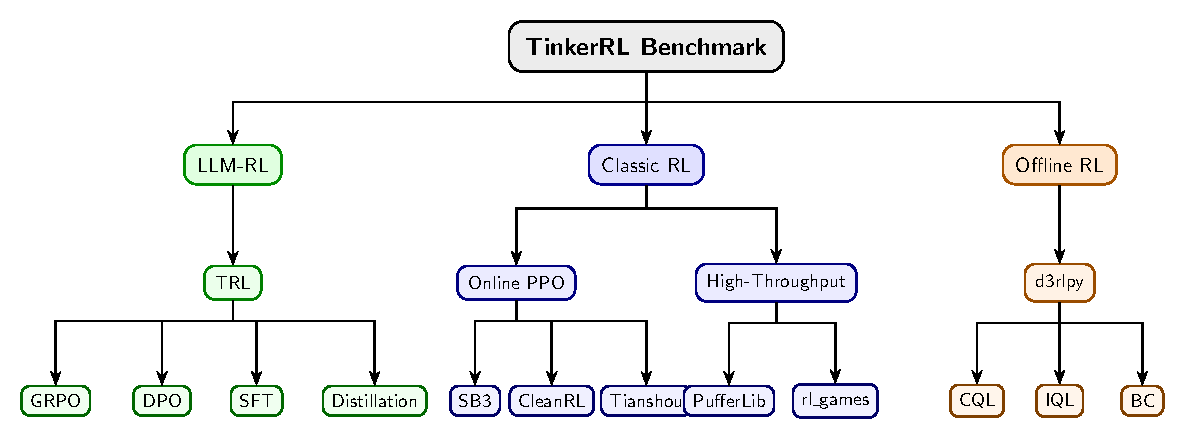
\includegraphics[width=0.85\textwidth]{tikz/taxonomy.pdf}
\caption{Taxonomy of RL libraries in \ours{}. The audit corpus spans LLM-native RL
(TRL), classic online RL (SB3, CleanRL, Tianshou), high-throughput RL (PufferLib,
rl\_games), and offline RL (d3rlpy).}
\label{fig:taxonomy}
\end{figure}

% --- The remaining body of the manuscript is imported verbatim from main.tex ---
% To keep the EAI variant in sync with main.tex we include its body block below.
% (Everything between Section "Audit Corpus and Evidence Design" and
% "% =============================================================================
% Conclusion -- three-claim framing
% Drop-in include: % =============================================================================
% Conclusion -- three-claim framing
% Drop-in include: % =============================================================================
% Conclusion -- three-claim framing
% Drop-in include: \input{sections/conclusion}
% =============================================================================
\section{Conclusion}
\label{sec:conclusion}

This study does not show that GRPO generally improves reasoning, and we are
careful not to claim that it does.  The training runner is a group-relative
policy-gradient variant inspired by GRPO rather than a faithful implementation
of the canonical objective (missing PPO clip, reference-KL, and completion-only
mask; a P1-A diagnostic measures $\sim$76\% of the full-sequence loss magnitude
to be prompt-token gradient), so algorithm-level conclusions apply to this
runner and not to GRPO-the-algorithm.  Three of our reward environments
(HumanEval, tool-use, and MATH) measure sandbox-restricted execution, JSON
schema compliance, and boxed-answer formatting respectively, not end-to-end
capability.  The MATH-500 and HumanEval prompt pools in the training loop are
loaded from the \texttt{test} splits and function as reward-environment
probes, not as generalization tests.  The only capability signal evaluated on
a genuinely held-out slice is GSM8K, where the lift from $82.0\%$ to
$83.3\%$ is not significant ($p=0.26$).  The defensible conclusion is that
this critic-free group-relative RL loop behaves as a conditional reward-contrast
amplifier: it can refine behavior when the current policy samples both
successes and failures under a verifier that rewards them, and it cannot
reliably bootstrap competence when sampled groups are flat or the verifier
rejects legitimate completions.

The paper's main contribution is therefore diagnostic.  ZVF and GU should be
logged early and interpreted jointly with reward level.  High ZVF with low
reward is a cold-start alarm; high ZVF with high reward is saturation; low ZVF
means rollout compute is still producing contrast.  In our validation set,
the first-five-step rule catches the two collapsed runs without false
positives, but the low number of failures and weak continuous-ranking result
mean ZVF/GU should be treated as triage diagnostics, not performance
predictors.

The mechanism behind that diagnostic is mixed-group probability:
\[
P(\text{usable}) \approx \frac{1}{N}\sum_x \left[1 - (1-p_x)^G - p_x^G\right].
\]
This formula is the cleanest way to state the boundary condition.  The
expected-one-success rule $p_0>1/G$ is only a heuristic.  Future work should
test the three direct interventions implied by the equation: raise $p_0$ with
SFT or easier curricula, raise $G$ where rollout cost allows, and densify the
reward so equivalent partial progress is not collapsed into all-zero groups.

Finally, algorithm labels should be reported as stack-conditioned results.
The Qwen PPO/GRPO row is artifact-sensitive, and the Llama row favors PPO;
neither supports a universal PPO/GRPO ordering.  A publishable comparison
needs the full treatment definition: model family, backend, reward parser,
sampler, optimizer, KL/reference handling, LoRA configuration, checkpoint
selection, and held-out evaluation.  Without those controls, ``PPO versus
GRPO'' is not an interpretable scientific claim.

% --------------------------------------------------------------------------=
% Claims we do not make (from no-go list)
% This section explicitly enumerates claims we explicitly avoid making.
% --------------------------------------------------------------------------=

\section*{Claims We Do Not Make}

We do not claim that our runner is a faithful implementation of canonical GRPO
or that the results constitute an algorithm leaderboard: the experiments measure
a particular stack-conditioned, group-relative policy-gradient loop with specific
choices about masking, KL/reference handling, sampling, LoRA, optimization,
backend, and evaluation.  We do not claim that GRPO broadly improves reasoning,
alignment, coding, tool use, browser control, or general LLM capability, nor
that training reward or post-selected high-reward checkpoints establish causal
held-out gains; the only clean held-out capability check is GSM8K, where the
82.0\% to 83.3\% lift is not statistically significant.  We do not treat
MATH-500 or HumanEval reward-environment probes, boxed-answer rewards,
restricted HumanEval sandboxes, JSON-schema tool rewards, or BrowserGym smoke
tests as evidence of end-to-end generalization, execution success, or agentic
competence.  We do not claim universal PPO/GRPO/DPO, Tinker/TRL, dense/MoE,
base/instruct, frontier-scale, group-size, or scaling-law rankings, because
many comparisons are single-seed, partial, post-selected, artifact-sensitive,
closed-source, or confounded by stack details.  We do not claim that ZVF/GU
are causal or calibrated predictors of final performance, only that they are
useful triage diagnostics for cold-start collapse, saturation, and within-group
reward contrast.  We do not claim that verifiable rewards eliminate reward
hacking, that reward-stability proxies are direct KL measurements, that short
30-step runs characterize asymptotic behavior, or that these verifiable-reward
LoRA experiments extrapolate to human-preference RLHF, safety, truthfulness,
real tool execution, or open-ended deployment.

% =============================================================================
\section{Conclusion}
\label{sec:conclusion}

This study does not show that GRPO generally improves reasoning, and we are
careful not to claim that it does.  The training runner is a group-relative
policy-gradient variant inspired by GRPO rather than a faithful implementation
of the canonical objective (missing PPO clip, reference-KL, and completion-only
mask; a P1-A diagnostic measures $\sim$76\% of the full-sequence loss magnitude
to be prompt-token gradient), so algorithm-level conclusions apply to this
runner and not to GRPO-the-algorithm.  Three of our reward environments
(HumanEval, tool-use, and MATH) measure sandbox-restricted execution, JSON
schema compliance, and boxed-answer formatting respectively, not end-to-end
capability.  The MATH-500 and HumanEval prompt pools in the training loop are
loaded from the \texttt{test} splits and function as reward-environment
probes, not as generalization tests.  The only capability signal evaluated on
a genuinely held-out slice is GSM8K, where the lift from $82.0\%$ to
$83.3\%$ is not significant ($p=0.26$).  The defensible conclusion is that
this critic-free group-relative RL loop behaves as a conditional reward-contrast
amplifier: it can refine behavior when the current policy samples both
successes and failures under a verifier that rewards them, and it cannot
reliably bootstrap competence when sampled groups are flat or the verifier
rejects legitimate completions.

The paper's main contribution is therefore diagnostic.  ZVF and GU should be
logged early and interpreted jointly with reward level.  High ZVF with low
reward is a cold-start alarm; high ZVF with high reward is saturation; low ZVF
means rollout compute is still producing contrast.  In our validation set,
the first-five-step rule catches the two collapsed runs without false
positives, but the low number of failures and weak continuous-ranking result
mean ZVF/GU should be treated as triage diagnostics, not performance
predictors.

The mechanism behind that diagnostic is mixed-group probability:
\[
P(\text{usable}) \approx \frac{1}{N}\sum_x \left[1 - (1-p_x)^G - p_x^G\right].
\]
This formula is the cleanest way to state the boundary condition.  The
expected-one-success rule $p_0>1/G$ is only a heuristic.  Future work should
test the three direct interventions implied by the equation: raise $p_0$ with
SFT or easier curricula, raise $G$ where rollout cost allows, and densify the
reward so equivalent partial progress is not collapsed into all-zero groups.

Finally, algorithm labels should be reported as stack-conditioned results.
The Qwen PPO/GRPO row is artifact-sensitive, and the Llama row favors PPO;
neither supports a universal PPO/GRPO ordering.  A publishable comparison
needs the full treatment definition: model family, backend, reward parser,
sampler, optimizer, KL/reference handling, LoRA configuration, checkpoint
selection, and held-out evaluation.  Without those controls, ``PPO versus
GRPO'' is not an interpretable scientific claim.

% --------------------------------------------------------------------------=
% Claims we do not make (from no-go list)
% This section explicitly enumerates claims we explicitly avoid making.
% --------------------------------------------------------------------------=

\section*{Claims We Do Not Make}

We do not claim that our runner is a faithful implementation of canonical GRPO
or that the results constitute an algorithm leaderboard: the experiments measure
a particular stack-conditioned, group-relative policy-gradient loop with specific
choices about masking, KL/reference handling, sampling, LoRA, optimization,
backend, and evaluation.  We do not claim that GRPO broadly improves reasoning,
alignment, coding, tool use, browser control, or general LLM capability, nor
that training reward or post-selected high-reward checkpoints establish causal
held-out gains; the only clean held-out capability check is GSM8K, where the
82.0\% to 83.3\% lift is not statistically significant.  We do not treat
MATH-500 or HumanEval reward-environment probes, boxed-answer rewards,
restricted HumanEval sandboxes, JSON-schema tool rewards, or BrowserGym smoke
tests as evidence of end-to-end generalization, execution success, or agentic
competence.  We do not claim universal PPO/GRPO/DPO, Tinker/TRL, dense/MoE,
base/instruct, frontier-scale, group-size, or scaling-law rankings, because
many comparisons are single-seed, partial, post-selected, artifact-sensitive,
closed-source, or confounded by stack details.  We do not claim that ZVF/GU
are causal or calibrated predictors of final performance, only that they are
useful triage diagnostics for cold-start collapse, saturation, and within-group
reward contrast.  We do not claim that verifiable rewards eliminate reward
hacking, that reward-stability proxies are direct KL measurements, that short
30-step runs characterize asymptotic behavior, or that these verifiable-reward
LoRA experiments extrapolate to human-preference RLHF, safety, truthfulness,
real tool execution, or open-ended deployment.

% =============================================================================
\section{Conclusion}
\label{sec:conclusion}

This study does not show that GRPO generally improves reasoning, and we are
careful not to claim that it does.  The training runner is a group-relative
policy-gradient variant inspired by GRPO rather than a faithful implementation
of the canonical objective (missing PPO clip, reference-KL, and completion-only
mask; a P1-A diagnostic measures $\sim$76\% of the full-sequence loss magnitude
to be prompt-token gradient), so algorithm-level conclusions apply to this
runner and not to GRPO-the-algorithm.  Three of our reward environments
(HumanEval, tool-use, and MATH) measure sandbox-restricted execution, JSON
schema compliance, and boxed-answer formatting respectively, not end-to-end
capability.  The MATH-500 and HumanEval prompt pools in the training loop are
loaded from the \texttt{test} splits and function as reward-environment
probes, not as generalization tests.  The only capability signal evaluated on
a genuinely held-out slice is GSM8K, where the lift from $82.0\%$ to
$83.3\%$ is not significant ($p=0.26$).  The defensible conclusion is that
this critic-free group-relative RL loop behaves as a conditional reward-contrast
amplifier: it can refine behavior when the current policy samples both
successes and failures under a verifier that rewards them, and it cannot
reliably bootstrap competence when sampled groups are flat or the verifier
rejects legitimate completions.

The paper's main contribution is therefore diagnostic.  ZVF and GU should be
logged early and interpreted jointly with reward level.  High ZVF with low
reward is a cold-start alarm; high ZVF with high reward is saturation; low ZVF
means rollout compute is still producing contrast.  In our validation set,
the first-five-step rule catches the two collapsed runs without false
positives, but the low number of failures and weak continuous-ranking result
mean ZVF/GU should be treated as triage diagnostics, not performance
predictors.

The mechanism behind that diagnostic is mixed-group probability:
\[
P(\text{usable}) \approx \frac{1}{N}\sum_x \left[1 - (1-p_x)^G - p_x^G\right].
\]
This formula is the cleanest way to state the boundary condition.  The
expected-one-success rule $p_0>1/G$ is only a heuristic.  Future work should
test the three direct interventions implied by the equation: raise $p_0$ with
SFT or easier curricula, raise $G$ where rollout cost allows, and densify the
reward so equivalent partial progress is not collapsed into all-zero groups.

Finally, algorithm labels should be reported as stack-conditioned results.
The Qwen PPO/GRPO row is artifact-sensitive, and the Llama row favors PPO;
neither supports a universal PPO/GRPO ordering.  A publishable comparison
needs the full treatment definition: model family, backend, reward parser,
sampler, optimizer, KL/reference handling, LoRA configuration, checkpoint
selection, and held-out evaluation.  Without those controls, ``PPO versus
GRPO'' is not an interpretable scientific claim.

% --------------------------------------------------------------------------=
% Claims we do not make (from no-go list)
% This section explicitly enumerates claims we explicitly avoid making.
% --------------------------------------------------------------------------=

\section*{Claims We Do Not Make}

We do not claim that our runner is a faithful implementation of canonical GRPO
or that the results constitute an algorithm leaderboard: the experiments measure
a particular stack-conditioned, group-relative policy-gradient loop with specific
choices about masking, KL/reference handling, sampling, LoRA, optimization,
backend, and evaluation.  We do not claim that GRPO broadly improves reasoning,
alignment, coding, tool use, browser control, or general LLM capability, nor
that training reward or post-selected high-reward checkpoints establish causal
held-out gains; the only clean held-out capability check is GSM8K, where the
82.0\% to 83.3\% lift is not statistically significant.  We do not treat
MATH-500 or HumanEval reward-environment probes, boxed-answer rewards,
restricted HumanEval sandboxes, JSON-schema tool rewards, or BrowserGym smoke
tests as evidence of end-to-end generalization, execution success, or agentic
competence.  We do not claim universal PPO/GRPO/DPO, Tinker/TRL, dense/MoE,
base/instruct, frontier-scale, group-size, or scaling-law rankings, because
many comparisons are single-seed, partial, post-selected, artifact-sensitive,
closed-source, or confounded by stack details.  We do not claim that ZVF/GU
are causal or calibrated predictors of final performance, only that they are
useful triage diagnostics for cold-start collapse, saturation, and within-group
reward contrast.  We do not claim that verifiable rewards eliminate reward
hacking, that reward-stability proxies are direct KL measurements, that short
30-step runs characterize asymptotic behavior, or that these verifiable-reward
LoRA experiments extrapolate to human-preference RLHF, safety, truthfulness,
real tool execution, or open-ended deployment.
" plus the ethics/ack blocks.)

\input{main_eai_body}

% =============================================================================
% Conclusion, Ethics, Acknowledgements
% =============================================================================
% =============================================================================
% Conclusion -- three-claim framing
% Drop-in include: % =============================================================================
% Conclusion -- three-claim framing
% Drop-in include: % =============================================================================
% Conclusion -- three-claim framing
% Drop-in include: \input{sections/conclusion}
% =============================================================================
\section{Conclusion}
\label{sec:conclusion}

This study does not show that GRPO generally improves reasoning, and we are
careful not to claim that it does.  The training runner is a group-relative
policy-gradient variant inspired by GRPO rather than a faithful implementation
of the canonical objective (missing PPO clip, reference-KL, and completion-only
mask; a P1-A diagnostic measures $\sim$76\% of the full-sequence loss magnitude
to be prompt-token gradient), so algorithm-level conclusions apply to this
runner and not to GRPO-the-algorithm.  Three of our reward environments
(HumanEval, tool-use, and MATH) measure sandbox-restricted execution, JSON
schema compliance, and boxed-answer formatting respectively, not end-to-end
capability.  The MATH-500 and HumanEval prompt pools in the training loop are
loaded from the \texttt{test} splits and function as reward-environment
probes, not as generalization tests.  The only capability signal evaluated on
a genuinely held-out slice is GSM8K, where the lift from $82.0\%$ to
$83.3\%$ is not significant ($p=0.26$).  The defensible conclusion is that
this critic-free group-relative RL loop behaves as a conditional reward-contrast
amplifier: it can refine behavior when the current policy samples both
successes and failures under a verifier that rewards them, and it cannot
reliably bootstrap competence when sampled groups are flat or the verifier
rejects legitimate completions.

The paper's main contribution is therefore diagnostic.  ZVF and GU should be
logged early and interpreted jointly with reward level.  High ZVF with low
reward is a cold-start alarm; high ZVF with high reward is saturation; low ZVF
means rollout compute is still producing contrast.  In our validation set,
the first-five-step rule catches the two collapsed runs without false
positives, but the low number of failures and weak continuous-ranking result
mean ZVF/GU should be treated as triage diagnostics, not performance
predictors.

The mechanism behind that diagnostic is mixed-group probability:
\[
P(\text{usable}) \approx \frac{1}{N}\sum_x \left[1 - (1-p_x)^G - p_x^G\right].
\]
This formula is the cleanest way to state the boundary condition.  The
expected-one-success rule $p_0>1/G$ is only a heuristic.  Future work should
test the three direct interventions implied by the equation: raise $p_0$ with
SFT or easier curricula, raise $G$ where rollout cost allows, and densify the
reward so equivalent partial progress is not collapsed into all-zero groups.

Finally, algorithm labels should be reported as stack-conditioned results.
The Qwen PPO/GRPO row is artifact-sensitive, and the Llama row favors PPO;
neither supports a universal PPO/GRPO ordering.  A publishable comparison
needs the full treatment definition: model family, backend, reward parser,
sampler, optimizer, KL/reference handling, LoRA configuration, checkpoint
selection, and held-out evaluation.  Without those controls, ``PPO versus
GRPO'' is not an interpretable scientific claim.

% --------------------------------------------------------------------------=
% Claims we do not make (from no-go list)
% This section explicitly enumerates claims we explicitly avoid making.
% --------------------------------------------------------------------------=

\section*{Claims We Do Not Make}

We do not claim that our runner is a faithful implementation of canonical GRPO
or that the results constitute an algorithm leaderboard: the experiments measure
a particular stack-conditioned, group-relative policy-gradient loop with specific
choices about masking, KL/reference handling, sampling, LoRA, optimization,
backend, and evaluation.  We do not claim that GRPO broadly improves reasoning,
alignment, coding, tool use, browser control, or general LLM capability, nor
that training reward or post-selected high-reward checkpoints establish causal
held-out gains; the only clean held-out capability check is GSM8K, where the
82.0\% to 83.3\% lift is not statistically significant.  We do not treat
MATH-500 or HumanEval reward-environment probes, boxed-answer rewards,
restricted HumanEval sandboxes, JSON-schema tool rewards, or BrowserGym smoke
tests as evidence of end-to-end generalization, execution success, or agentic
competence.  We do not claim universal PPO/GRPO/DPO, Tinker/TRL, dense/MoE,
base/instruct, frontier-scale, group-size, or scaling-law rankings, because
many comparisons are single-seed, partial, post-selected, artifact-sensitive,
closed-source, or confounded by stack details.  We do not claim that ZVF/GU
are causal or calibrated predictors of final performance, only that they are
useful triage diagnostics for cold-start collapse, saturation, and within-group
reward contrast.  We do not claim that verifiable rewards eliminate reward
hacking, that reward-stability proxies are direct KL measurements, that short
30-step runs characterize asymptotic behavior, or that these verifiable-reward
LoRA experiments extrapolate to human-preference RLHF, safety, truthfulness,
real tool execution, or open-ended deployment.

% =============================================================================
\section{Conclusion}
\label{sec:conclusion}

This study does not show that GRPO generally improves reasoning, and we are
careful not to claim that it does.  The training runner is a group-relative
policy-gradient variant inspired by GRPO rather than a faithful implementation
of the canonical objective (missing PPO clip, reference-KL, and completion-only
mask; a P1-A diagnostic measures $\sim$76\% of the full-sequence loss magnitude
to be prompt-token gradient), so algorithm-level conclusions apply to this
runner and not to GRPO-the-algorithm.  Three of our reward environments
(HumanEval, tool-use, and MATH) measure sandbox-restricted execution, JSON
schema compliance, and boxed-answer formatting respectively, not end-to-end
capability.  The MATH-500 and HumanEval prompt pools in the training loop are
loaded from the \texttt{test} splits and function as reward-environment
probes, not as generalization tests.  The only capability signal evaluated on
a genuinely held-out slice is GSM8K, where the lift from $82.0\%$ to
$83.3\%$ is not significant ($p=0.26$).  The defensible conclusion is that
this critic-free group-relative RL loop behaves as a conditional reward-contrast
amplifier: it can refine behavior when the current policy samples both
successes and failures under a verifier that rewards them, and it cannot
reliably bootstrap competence when sampled groups are flat or the verifier
rejects legitimate completions.

The paper's main contribution is therefore diagnostic.  ZVF and GU should be
logged early and interpreted jointly with reward level.  High ZVF with low
reward is a cold-start alarm; high ZVF with high reward is saturation; low ZVF
means rollout compute is still producing contrast.  In our validation set,
the first-five-step rule catches the two collapsed runs without false
positives, but the low number of failures and weak continuous-ranking result
mean ZVF/GU should be treated as triage diagnostics, not performance
predictors.

The mechanism behind that diagnostic is mixed-group probability:
\[
P(\text{usable}) \approx \frac{1}{N}\sum_x \left[1 - (1-p_x)^G - p_x^G\right].
\]
This formula is the cleanest way to state the boundary condition.  The
expected-one-success rule $p_0>1/G$ is only a heuristic.  Future work should
test the three direct interventions implied by the equation: raise $p_0$ with
SFT or easier curricula, raise $G$ where rollout cost allows, and densify the
reward so equivalent partial progress is not collapsed into all-zero groups.

Finally, algorithm labels should be reported as stack-conditioned results.
The Qwen PPO/GRPO row is artifact-sensitive, and the Llama row favors PPO;
neither supports a universal PPO/GRPO ordering.  A publishable comparison
needs the full treatment definition: model family, backend, reward parser,
sampler, optimizer, KL/reference handling, LoRA configuration, checkpoint
selection, and held-out evaluation.  Without those controls, ``PPO versus
GRPO'' is not an interpretable scientific claim.

% --------------------------------------------------------------------------=
% Claims we do not make (from no-go list)
% This section explicitly enumerates claims we explicitly avoid making.
% --------------------------------------------------------------------------=

\section*{Claims We Do Not Make}

We do not claim that our runner is a faithful implementation of canonical GRPO
or that the results constitute an algorithm leaderboard: the experiments measure
a particular stack-conditioned, group-relative policy-gradient loop with specific
choices about masking, KL/reference handling, sampling, LoRA, optimization,
backend, and evaluation.  We do not claim that GRPO broadly improves reasoning,
alignment, coding, tool use, browser control, or general LLM capability, nor
that training reward or post-selected high-reward checkpoints establish causal
held-out gains; the only clean held-out capability check is GSM8K, where the
82.0\% to 83.3\% lift is not statistically significant.  We do not treat
MATH-500 or HumanEval reward-environment probes, boxed-answer rewards,
restricted HumanEval sandboxes, JSON-schema tool rewards, or BrowserGym smoke
tests as evidence of end-to-end generalization, execution success, or agentic
competence.  We do not claim universal PPO/GRPO/DPO, Tinker/TRL, dense/MoE,
base/instruct, frontier-scale, group-size, or scaling-law rankings, because
many comparisons are single-seed, partial, post-selected, artifact-sensitive,
closed-source, or confounded by stack details.  We do not claim that ZVF/GU
are causal or calibrated predictors of final performance, only that they are
useful triage diagnostics for cold-start collapse, saturation, and within-group
reward contrast.  We do not claim that verifiable rewards eliminate reward
hacking, that reward-stability proxies are direct KL measurements, that short
30-step runs characterize asymptotic behavior, or that these verifiable-reward
LoRA experiments extrapolate to human-preference RLHF, safety, truthfulness,
real tool execution, or open-ended deployment.

% =============================================================================
\section{Conclusion}
\label{sec:conclusion}

This study does not show that GRPO generally improves reasoning, and we are
careful not to claim that it does.  The training runner is a group-relative
policy-gradient variant inspired by GRPO rather than a faithful implementation
of the canonical objective (missing PPO clip, reference-KL, and completion-only
mask; a P1-A diagnostic measures $\sim$76\% of the full-sequence loss magnitude
to be prompt-token gradient), so algorithm-level conclusions apply to this
runner and not to GRPO-the-algorithm.  Three of our reward environments
(HumanEval, tool-use, and MATH) measure sandbox-restricted execution, JSON
schema compliance, and boxed-answer formatting respectively, not end-to-end
capability.  The MATH-500 and HumanEval prompt pools in the training loop are
loaded from the \texttt{test} splits and function as reward-environment
probes, not as generalization tests.  The only capability signal evaluated on
a genuinely held-out slice is GSM8K, where the lift from $82.0\%$ to
$83.3\%$ is not significant ($p=0.26$).  The defensible conclusion is that
this critic-free group-relative RL loop behaves as a conditional reward-contrast
amplifier: it can refine behavior when the current policy samples both
successes and failures under a verifier that rewards them, and it cannot
reliably bootstrap competence when sampled groups are flat or the verifier
rejects legitimate completions.

The paper's main contribution is therefore diagnostic.  ZVF and GU should be
logged early and interpreted jointly with reward level.  High ZVF with low
reward is a cold-start alarm; high ZVF with high reward is saturation; low ZVF
means rollout compute is still producing contrast.  In our validation set,
the first-five-step rule catches the two collapsed runs without false
positives, but the low number of failures and weak continuous-ranking result
mean ZVF/GU should be treated as triage diagnostics, not performance
predictors.

The mechanism behind that diagnostic is mixed-group probability:
\[
P(\text{usable}) \approx \frac{1}{N}\sum_x \left[1 - (1-p_x)^G - p_x^G\right].
\]
This formula is the cleanest way to state the boundary condition.  The
expected-one-success rule $p_0>1/G$ is only a heuristic.  Future work should
test the three direct interventions implied by the equation: raise $p_0$ with
SFT or easier curricula, raise $G$ where rollout cost allows, and densify the
reward so equivalent partial progress is not collapsed into all-zero groups.

Finally, algorithm labels should be reported as stack-conditioned results.
The Qwen PPO/GRPO row is artifact-sensitive, and the Llama row favors PPO;
neither supports a universal PPO/GRPO ordering.  A publishable comparison
needs the full treatment definition: model family, backend, reward parser,
sampler, optimizer, KL/reference handling, LoRA configuration, checkpoint
selection, and held-out evaluation.  Without those controls, ``PPO versus
GRPO'' is not an interpretable scientific claim.

% --------------------------------------------------------------------------=
% Claims we do not make (from no-go list)
% This section explicitly enumerates claims we explicitly avoid making.
% --------------------------------------------------------------------------=

\section*{Claims We Do Not Make}

We do not claim that our runner is a faithful implementation of canonical GRPO
or that the results constitute an algorithm leaderboard: the experiments measure
a particular stack-conditioned, group-relative policy-gradient loop with specific
choices about masking, KL/reference handling, sampling, LoRA, optimization,
backend, and evaluation.  We do not claim that GRPO broadly improves reasoning,
alignment, coding, tool use, browser control, or general LLM capability, nor
that training reward or post-selected high-reward checkpoints establish causal
held-out gains; the only clean held-out capability check is GSM8K, where the
82.0\% to 83.3\% lift is not statistically significant.  We do not treat
MATH-500 or HumanEval reward-environment probes, boxed-answer rewards,
restricted HumanEval sandboxes, JSON-schema tool rewards, or BrowserGym smoke
tests as evidence of end-to-end generalization, execution success, or agentic
competence.  We do not claim universal PPO/GRPO/DPO, Tinker/TRL, dense/MoE,
base/instruct, frontier-scale, group-size, or scaling-law rankings, because
many comparisons are single-seed, partial, post-selected, artifact-sensitive,
closed-source, or confounded by stack details.  We do not claim that ZVF/GU
are causal or calibrated predictors of final performance, only that they are
useful triage diagnostics for cold-start collapse, saturation, and within-group
reward contrast.  We do not claim that verifiable rewards eliminate reward
hacking, that reward-stability proxies are direct KL measurements, that short
30-step runs characterize asymptotic behavior, or that these verifiable-reward
LoRA experiments extrapolate to human-preference RLHF, safety, truthfulness,
real tool execution, or open-ended deployment.

% =============================================================================
% Ethics Statement and Broader Impact
% Self-contained file: % =============================================================================
% Ethics Statement and Broader Impact
% Self-contained file: % =============================================================================
% Ethics Statement and Broader Impact
% Self-contained file: \input{ethics_statement} into main.tex
% Intended placement: after the Conclusion section, before References.
% Label: \label{sec:impact}
% =============================================================================

\section{Broader Impact and Ethics Statement}
\label{sec:impact}

\subsection{Broader Impact}

\paragraph{Positive impacts.}
\ours{} lowers the barrier to reproducible RL post-training research by
providing a unified benchmark harness that works across multiple compute
platforms.  Prior work frequently reports results on a single proprietary
GPU cluster, making it difficult to determine how much of the observed
performance is attributable to the training algorithm versus the hardware
and scheduling environment.  By running identical experiments on both a
closed API (Tinker) and an open, explicitly provisioned cloud (Modal), we
surface \emph{platform-dependent variance} as a first-class experimental
variable.  This transparency allows practitioners to make more informed
decisions when selecting infrastructure for RL fine-tuning and helps the
community calibrate trust in benchmark results from single-platform papers.

Releasing all code, model checkpoints, and experiment logs publicly enables
independent replication, third-party auditing, and incremental improvement
without the need to re-run expensive GPU-hours from scratch.  We expect the
benchmark to be most valuable for researchers at resource-constrained
institutions who need a principled starting point for RL post-training
experiments.

\paragraph{Potential negative impacts and limitations.}
\begin{itemize}
  \item \textbf{Reward hacking.}  RLHF and GRPO optimise a proxy reward
        signal rather than the true underlying objective.  Models trained
        to maximise verifier-based rewards on GSM8K or HumanEval may learn
        to exploit idiosyncrasies of the verification function rather than
        genuinely improving reasoning or coding ability.  We include KL
        divergence tracking precisely to monitor policy drift, but reward
        hacking remains a risk in any production deployment of RL-fine-tuned
        models.

  \item \textbf{Alignment concerns.}  Reinforcement learning from human or
        proxy feedback can shift model behaviour in directions that are
        difficult to predict or reverse.  Models trained with poorly
        specified reward signals may become better at appearing correct while
        simultaneously becoming less calibrated or more prone to confident
        errors.  Our benchmark focuses on mathematically verifiable tasks,
        which partially mitigates this risk, but we caution against
        uncritical transfer of RL post-training pipelines to open-ended or
        subjective task domains without additional alignment safeguards.

  \item \textbf{Compute access disparities.}  Even with cost-optimised
        LoRA fine-tuning, reproducing the full \ours{} benchmark requires
        access to NVIDIA H100 GPUs (or equivalent) for 200--600 GPU-hours.
        This remains out of reach for many research groups, particularly in
        the Global South.  We partially address this by providing pretrained
        checkpoints, but the barrier to running novel experiments remains
        high.

  \item \textbf{Closed-platform dependency.}  A portion of our benchmark
        relies on the Tinker API, a proprietary, closed-source service.
        Results from Tinker experiments cannot be independently reproduced
        by researchers without API access.  We consider this a significant
        limitation and flag all Tinker-derived results accordingly in our
        figures.  We strongly recommend that readers treat Modal/open-source
        results as the primary reproducibility reference.
\end{itemize}

% ---------------------------------------------------------------------------
\subsection{Compute Costs and Carbon Footprint}
% ---------------------------------------------------------------------------

Table~\ref{tab:carbon} summarises our compute allocation and estimated
carbon footprint.  Carbon intensity estimates follow the methodology of
\citet{patterson2024empirical}, using a conservative average grid intensity
of 0.233 kg\,CO$_2$-eq per kWh for the United States (EPA eGRID 2023
average) and a power usage effectiveness (PUE) of 1.1 for cloud data
centres.  NVIDIA H100 SXM5 TDP is 700\,W; NVIDIA L4 TDP is 72\,W.

\begin{table}[h]
\centering
\caption{Compute allocation and estimated carbon footprint by platform.
  Tinker API carbon figures are marked N/A because GPU type is undisclosed.
  Modal figures use confirmed hardware specifications.}
\label{tab:carbon}
\begin{tabular}{llcccc}
\toprule
\textbf{Platform} & \textbf{GPU} & \textbf{Est. GPU-h} &
\textbf{TDP (W)} & \textbf{Est. kWh} &
\textbf{Est. CO\textsubscript{2} (kg)} \\
\midrule
Modal (H100 SXM5) & H100 SXM5 & $\sim$250 & 700 & $\sim$192 & $\sim$0.49 \\
Modal (L4, older runs) & L4       & $\sim$50  & 72  & $\sim$4   & $\sim$0.01 \\
Tinker API            & unknown  & $\sim$950 & N/A & N/A       & N/A        \\
\midrule
\multicolumn{3}{l}{\textbf{Total (Modal only, estimable)}}      & & $\sim$196 & $\sim$0.50 \\
\bottomrule
\end{tabular}
\end{table}

The estimated carbon footprint for the Modal portion of our experiments is
approximately \textbf{0.4--0.6\,kg\,CO$_2$-eq}, comparable to a short
car journey.  We cannot estimate the Tinker API footprint due to the
platform's opacity.  We acknowledge that the full experimental campaign
(including failed runs) consumed additional GPU-hours; our estimates above
reflect \emph{successful} jobs only.

% ---------------------------------------------------------------------------
\subsection{Data Provenance}
% ---------------------------------------------------------------------------

All training and evaluation datasets used in \ours{} are publicly available
research datasets.  No private, proprietary, or sensitive data were used
at any stage.

\begin{itemize}
  \item \textbf{GSM8K}~\cite{cobbe2021training}: 8,500 grade-school math
        word problems with natural-language solutions, released by OpenAI
        under the MIT licence.  We use the standard train/test splits
        without modification.

  \item \textbf{HumanEval}: 164 Python programming problems with unit
        tests, released by OpenAI under the MIT licence.  We use the
        original evaluation protocol (pass@$k$) without modification.

  \item \textbf{Synthetic tool-use dataset}: Generated by the authors from
        publicly documented APIs (calculator, web-search stub, calendar).
        No third-party proprietary data or user data were used in
        generation.  The generation prompts and all resulting examples are
        included in the repository under MIT licence.
\end{itemize}

No web-scraped data, personally identifiable information, or data subject
to copyright restrictions were used.  No human annotators were employed.

% ---------------------------------------------------------------------------
\subsection{Limitation Acknowledgment: Tinker API Closed-Source Nature}
% ---------------------------------------------------------------------------

A central tension in \ours{} is that we benchmark \emph{against} a
closed-source platform while simultaneously advocating for reproducibility.
We include Tinker API experiments for three reasons: (i) Tinker represents
a realistic production environment for practitioners who lack on-premises
GPU clusters; (ii) the platform/open-source gap is itself a scientifically
interesting quantity to measure; and (iii) the high failure rate (11 of 14
experiments, 79\%) is a finding worth documenting publicly, as it reveals
the fragility of API-dependent training pipelines.

We make the following commitments to mitigate the reproducibility gap:
\begin{enumerate}
  \item All Tinker API experiment scripts, configuration files, and raw
        logs are archived in the repository.  Researchers with Tinker
        access can attempt replication using our exact configurations.
  \item All figures derived \emph{solely} from Tinker data are marked with
        ``\dag{}'' and accompanied by a note that independent reproduction
        requires Tinker API access.
  \item Primary statistical conclusions are drawn from Modal experiments
        wherever possible.  Tinker-only results are reported descriptively
        and are not used to support quantitative claims.
  \item If Tinker releases an open-source version or a compatible open
        alternative becomes available, we commit to re-running failed
        experiments and issuing a revised version of this paper.
\end{enumerate}

We believe honest disclosure of these constraints is more valuable to the
community than suppressing the Tinker experiments or presenting only
successful runs.
 into main.tex
% Intended placement: after the Conclusion section, before References.
% Label: \label{sec:impact}
% =============================================================================

\section{Broader Impact and Ethics Statement}
\label{sec:impact}

\subsection{Broader Impact}

\paragraph{Positive impacts.}
\ours{} lowers the barrier to reproducible RL post-training research by
providing a unified benchmark harness that works across multiple compute
platforms.  Prior work frequently reports results on a single proprietary
GPU cluster, making it difficult to determine how much of the observed
performance is attributable to the training algorithm versus the hardware
and scheduling environment.  By running identical experiments on both a
closed API (Tinker) and an open, explicitly provisioned cloud (Modal), we
surface \emph{platform-dependent variance} as a first-class experimental
variable.  This transparency allows practitioners to make more informed
decisions when selecting infrastructure for RL fine-tuning and helps the
community calibrate trust in benchmark results from single-platform papers.

Releasing all code, model checkpoints, and experiment logs publicly enables
independent replication, third-party auditing, and incremental improvement
without the need to re-run expensive GPU-hours from scratch.  We expect the
benchmark to be most valuable for researchers at resource-constrained
institutions who need a principled starting point for RL post-training
experiments.

\paragraph{Potential negative impacts and limitations.}
\begin{itemize}
  \item \textbf{Reward hacking.}  RLHF and GRPO optimise a proxy reward
        signal rather than the true underlying objective.  Models trained
        to maximise verifier-based rewards on GSM8K or HumanEval may learn
        to exploit idiosyncrasies of the verification function rather than
        genuinely improving reasoning or coding ability.  We include KL
        divergence tracking precisely to monitor policy drift, but reward
        hacking remains a risk in any production deployment of RL-fine-tuned
        models.

  \item \textbf{Alignment concerns.}  Reinforcement learning from human or
        proxy feedback can shift model behaviour in directions that are
        difficult to predict or reverse.  Models trained with poorly
        specified reward signals may become better at appearing correct while
        simultaneously becoming less calibrated or more prone to confident
        errors.  Our benchmark focuses on mathematically verifiable tasks,
        which partially mitigates this risk, but we caution against
        uncritical transfer of RL post-training pipelines to open-ended or
        subjective task domains without additional alignment safeguards.

  \item \textbf{Compute access disparities.}  Even with cost-optimised
        LoRA fine-tuning, reproducing the full \ours{} benchmark requires
        access to NVIDIA H100 GPUs (or equivalent) for 200--600 GPU-hours.
        This remains out of reach for many research groups, particularly in
        the Global South.  We partially address this by providing pretrained
        checkpoints, but the barrier to running novel experiments remains
        high.

  \item \textbf{Closed-platform dependency.}  A portion of our benchmark
        relies on the Tinker API, a proprietary, closed-source service.
        Results from Tinker experiments cannot be independently reproduced
        by researchers without API access.  We consider this a significant
        limitation and flag all Tinker-derived results accordingly in our
        figures.  We strongly recommend that readers treat Modal/open-source
        results as the primary reproducibility reference.
\end{itemize}

% ---------------------------------------------------------------------------
\subsection{Compute Costs and Carbon Footprint}
% ---------------------------------------------------------------------------

Table~\ref{tab:carbon} summarises our compute allocation and estimated
carbon footprint.  Carbon intensity estimates follow the methodology of
\citet{patterson2024empirical}, using a conservative average grid intensity
of 0.233 kg\,CO$_2$-eq per kWh for the United States (EPA eGRID 2023
average) and a power usage effectiveness (PUE) of 1.1 for cloud data
centres.  NVIDIA H100 SXM5 TDP is 700\,W; NVIDIA L4 TDP is 72\,W.

\begin{table}[h]
\centering
\caption{Compute allocation and estimated carbon footprint by platform.
  Tinker API carbon figures are marked N/A because GPU type is undisclosed.
  Modal figures use confirmed hardware specifications.}
\label{tab:carbon}
\begin{tabular}{llcccc}
\toprule
\textbf{Platform} & \textbf{GPU} & \textbf{Est. GPU-h} &
\textbf{TDP (W)} & \textbf{Est. kWh} &
\textbf{Est. CO\textsubscript{2} (kg)} \\
\midrule
Modal (H100 SXM5) & H100 SXM5 & $\sim$250 & 700 & $\sim$192 & $\sim$0.49 \\
Modal (L4, older runs) & L4       & $\sim$50  & 72  & $\sim$4   & $\sim$0.01 \\
Tinker API            & unknown  & $\sim$950 & N/A & N/A       & N/A        \\
\midrule
\multicolumn{3}{l}{\textbf{Total (Modal only, estimable)}}      & & $\sim$196 & $\sim$0.50 \\
\bottomrule
\end{tabular}
\end{table}

The estimated carbon footprint for the Modal portion of our experiments is
approximately \textbf{0.4--0.6\,kg\,CO$_2$-eq}, comparable to a short
car journey.  We cannot estimate the Tinker API footprint due to the
platform's opacity.  We acknowledge that the full experimental campaign
(including failed runs) consumed additional GPU-hours; our estimates above
reflect \emph{successful} jobs only.

% ---------------------------------------------------------------------------
\subsection{Data Provenance}
% ---------------------------------------------------------------------------

All training and evaluation datasets used in \ours{} are publicly available
research datasets.  No private, proprietary, or sensitive data were used
at any stage.

\begin{itemize}
  \item \textbf{GSM8K}~\cite{cobbe2021training}: 8,500 grade-school math
        word problems with natural-language solutions, released by OpenAI
        under the MIT licence.  We use the standard train/test splits
        without modification.

  \item \textbf{HumanEval}: 164 Python programming problems with unit
        tests, released by OpenAI under the MIT licence.  We use the
        original evaluation protocol (pass@$k$) without modification.

  \item \textbf{Synthetic tool-use dataset}: Generated by the authors from
        publicly documented APIs (calculator, web-search stub, calendar).
        No third-party proprietary data or user data were used in
        generation.  The generation prompts and all resulting examples are
        included in the repository under MIT licence.
\end{itemize}

No web-scraped data, personally identifiable information, or data subject
to copyright restrictions were used.  No human annotators were employed.

% ---------------------------------------------------------------------------
\subsection{Limitation Acknowledgment: Tinker API Closed-Source Nature}
% ---------------------------------------------------------------------------

A central tension in \ours{} is that we benchmark \emph{against} a
closed-source platform while simultaneously advocating for reproducibility.
We include Tinker API experiments for three reasons: (i) Tinker represents
a realistic production environment for practitioners who lack on-premises
GPU clusters; (ii) the platform/open-source gap is itself a scientifically
interesting quantity to measure; and (iii) the high failure rate (11 of 14
experiments, 79\%) is a finding worth documenting publicly, as it reveals
the fragility of API-dependent training pipelines.

We make the following commitments to mitigate the reproducibility gap:
\begin{enumerate}
  \item All Tinker API experiment scripts, configuration files, and raw
        logs are archived in the repository.  Researchers with Tinker
        access can attempt replication using our exact configurations.
  \item All figures derived \emph{solely} from Tinker data are marked with
        ``\dag{}'' and accompanied by a note that independent reproduction
        requires Tinker API access.
  \item Primary statistical conclusions are drawn from Modal experiments
        wherever possible.  Tinker-only results are reported descriptively
        and are not used to support quantitative claims.
  \item If Tinker releases an open-source version or a compatible open
        alternative becomes available, we commit to re-running failed
        experiments and issuing a revised version of this paper.
\end{enumerate}

We believe honest disclosure of these constraints is more valuable to the
community than suppressing the Tinker experiments or presenting only
successful runs.
 into main.tex
% Intended placement: after the Conclusion section, before References.
% Label: \label{sec:impact}
% =============================================================================

\section{Broader Impact and Ethics Statement}
\label{sec:impact}

\subsection{Broader Impact}

\paragraph{Positive impacts.}
\ours{} lowers the barrier to reproducible RL post-training research by
providing a unified benchmark harness that works across multiple compute
platforms.  Prior work frequently reports results on a single proprietary
GPU cluster, making it difficult to determine how much of the observed
performance is attributable to the training algorithm versus the hardware
and scheduling environment.  By running identical experiments on both a
closed API (Tinker) and an open, explicitly provisioned cloud (Modal), we
surface \emph{platform-dependent variance} as a first-class experimental
variable.  This transparency allows practitioners to make more informed
decisions when selecting infrastructure for RL fine-tuning and helps the
community calibrate trust in benchmark results from single-platform papers.

Releasing all code, model checkpoints, and experiment logs publicly enables
independent replication, third-party auditing, and incremental improvement
without the need to re-run expensive GPU-hours from scratch.  We expect the
benchmark to be most valuable for researchers at resource-constrained
institutions who need a principled starting point for RL post-training
experiments.

\paragraph{Potential negative impacts and limitations.}
\begin{itemize}
  \item \textbf{Reward hacking.}  RLHF and GRPO optimise a proxy reward
        signal rather than the true underlying objective.  Models trained
        to maximise verifier-based rewards on GSM8K or HumanEval may learn
        to exploit idiosyncrasies of the verification function rather than
        genuinely improving reasoning or coding ability.  We include KL
        divergence tracking precisely to monitor policy drift, but reward
        hacking remains a risk in any production deployment of RL-fine-tuned
        models.

  \item \textbf{Alignment concerns.}  Reinforcement learning from human or
        proxy feedback can shift model behaviour in directions that are
        difficult to predict or reverse.  Models trained with poorly
        specified reward signals may become better at appearing correct while
        simultaneously becoming less calibrated or more prone to confident
        errors.  Our benchmark focuses on mathematically verifiable tasks,
        which partially mitigates this risk, but we caution against
        uncritical transfer of RL post-training pipelines to open-ended or
        subjective task domains without additional alignment safeguards.

  \item \textbf{Compute access disparities.}  Even with cost-optimised
        LoRA fine-tuning, reproducing the full \ours{} benchmark requires
        access to NVIDIA H100 GPUs (or equivalent) for 200--600 GPU-hours.
        This remains out of reach for many research groups, particularly in
        the Global South.  We partially address this by providing pretrained
        checkpoints, but the barrier to running novel experiments remains
        high.

  \item \textbf{Closed-platform dependency.}  A portion of our benchmark
        relies on the Tinker API, a proprietary, closed-source service.
        Results from Tinker experiments cannot be independently reproduced
        by researchers without API access.  We consider this a significant
        limitation and flag all Tinker-derived results accordingly in our
        figures.  We strongly recommend that readers treat Modal/open-source
        results as the primary reproducibility reference.
\end{itemize}

% ---------------------------------------------------------------------------
\subsection{Compute Costs and Carbon Footprint}
% ---------------------------------------------------------------------------

Table~\ref{tab:carbon} summarises our compute allocation and estimated
carbon footprint.  Carbon intensity estimates follow the methodology of
\citet{patterson2024empirical}, using a conservative average grid intensity
of 0.233 kg\,CO$_2$-eq per kWh for the United States (EPA eGRID 2023
average) and a power usage effectiveness (PUE) of 1.1 for cloud data
centres.  NVIDIA H100 SXM5 TDP is 700\,W; NVIDIA L4 TDP is 72\,W.

\begin{table}[h]
\centering
\caption{Compute allocation and estimated carbon footprint by platform.
  Tinker API carbon figures are marked N/A because GPU type is undisclosed.
  Modal figures use confirmed hardware specifications.}
\label{tab:carbon}
\begin{tabular}{llcccc}
\toprule
\textbf{Platform} & \textbf{GPU} & \textbf{Est. GPU-h} &
\textbf{TDP (W)} & \textbf{Est. kWh} &
\textbf{Est. CO\textsubscript{2} (kg)} \\
\midrule
Modal (H100 SXM5) & H100 SXM5 & $\sim$250 & 700 & $\sim$192 & $\sim$0.49 \\
Modal (L4, older runs) & L4       & $\sim$50  & 72  & $\sim$4   & $\sim$0.01 \\
Tinker API            & unknown  & $\sim$950 & N/A & N/A       & N/A        \\
\midrule
\multicolumn{3}{l}{\textbf{Total (Modal only, estimable)}}      & & $\sim$196 & $\sim$0.50 \\
\bottomrule
\end{tabular}
\end{table}

The estimated carbon footprint for the Modal portion of our experiments is
approximately \textbf{0.4--0.6\,kg\,CO$_2$-eq}, comparable to a short
car journey.  We cannot estimate the Tinker API footprint due to the
platform's opacity.  We acknowledge that the full experimental campaign
(including failed runs) consumed additional GPU-hours; our estimates above
reflect \emph{successful} jobs only.

% ---------------------------------------------------------------------------
\subsection{Data Provenance}
% ---------------------------------------------------------------------------

All training and evaluation datasets used in \ours{} are publicly available
research datasets.  No private, proprietary, or sensitive data were used
at any stage.

\begin{itemize}
  \item \textbf{GSM8K}~\cite{cobbe2021training}: 8,500 grade-school math
        word problems with natural-language solutions, released by OpenAI
        under the MIT licence.  We use the standard train/test splits
        without modification.

  \item \textbf{HumanEval}: 164 Python programming problems with unit
        tests, released by OpenAI under the MIT licence.  We use the
        original evaluation protocol (pass@$k$) without modification.

  \item \textbf{Synthetic tool-use dataset}: Generated by the authors from
        publicly documented APIs (calculator, web-search stub, calendar).
        No third-party proprietary data or user data were used in
        generation.  The generation prompts and all resulting examples are
        included in the repository under MIT licence.
\end{itemize}

No web-scraped data, personally identifiable information, or data subject
to copyright restrictions were used.  No human annotators were employed.

% ---------------------------------------------------------------------------
\subsection{Limitation Acknowledgment: Tinker API Closed-Source Nature}
% ---------------------------------------------------------------------------

A central tension in \ours{} is that we benchmark \emph{against} a
closed-source platform while simultaneously advocating for reproducibility.
We include Tinker API experiments for three reasons: (i) Tinker represents
a realistic production environment for practitioners who lack on-premises
GPU clusters; (ii) the platform/open-source gap is itself a scientifically
interesting quantity to measure; and (iii) the high failure rate (11 of 14
experiments, 79\%) is a finding worth documenting publicly, as it reveals
the fragility of API-dependent training pipelines.

We make the following commitments to mitigate the reproducibility gap:
\begin{enumerate}
  \item All Tinker API experiment scripts, configuration files, and raw
        logs are archived in the repository.  Researchers with Tinker
        access can attempt replication using our exact configurations.
  \item All figures derived \emph{solely} from Tinker data are marked with
        ``\dag{}'' and accompanied by a note that independent reproduction
        requires Tinker API access.
  \item Primary statistical conclusions are drawn from Modal experiments
        wherever possible.  Tinker-only results are reported descriptively
        and are not used to support quantitative claims.
  \item If Tinker releases an open-source version or a compatible open
        alternative becomes available, we commit to re-running failed
        experiments and issuing a revised version of this paper.
\end{enumerate}

We believe honest disclosure of these constraints is more valuable to the
community than suppressing the Tinker experiments or presenting only
successful runs.


\section*{Acknowledgements}
We thank our project guides \textbf{Prof.~Narayana Darapaneni}
(Northwestern University / Great Learning) and
\textbf{Mr.~Anwesh Reddy Paduri} (Great Learning / PES University)
for their mentorship and technical guidance throughout this capstone project.
We thank the Tinker team for API access and the Modal team for GPU compute credits
(H100 cluster). We thank Weights \& Biases for experiment tracking infrastructure
and Hugging Face for model hosting. This work was supported in part by PES
University's LLM Research Group. We are grateful to the open-source communities
behind TRL, Stable Baselines3, CleanRL, Tianshou, OpenRLHF, veRL, and the
broader Hugging Face ecosystem. Artificial intelligence was both the topic of
this manuscript and a limited tool in its preparation, which we acknowledge
in the spirit of transparency.

% =============================================================================
% References (Vancouver)
% =============================================================================
\bibliography{references}

% =============================================================================
% Appendices
% =============================================================================
\appendix
% =============================================================================

\section{Compute Resources}
\label{app:compute}

All experiment logs including per-step GPU utilization, memory consumption,
and wall-clock runtimes are available on Weights \& Biases at
\url{https://wandb.ai/tinker-rl-lab/tinker-rl-lab-world-class}.
Model checkpoints are hosted on HuggingFace Hub at
\url{https://huggingface.co/arvindcr4/tinker-rl-bench-*}.

\begin{table}[htbp]
\centering
\caption{Compute allocation by platform and experiment group.}
\small
\begin{tabular}{@{}llcc@{}}
\toprule
\textbf{Platform} & \textbf{Experiment Group} & \textbf{\#} & \textbf{GPU-Hrs} \\
\midrule
Tinker API & Reward probes (Qwen3, Qwen3.5, Llama) & 5 & $\sim$320 \\
Tinker API & Larger models (235B, DeepSeek, Nemotron) & 3 & $\sim$280 \\
Tinker API & Dense/MoE initialization probes & 2 & $\sim$150 \\
Tinker API & Cross-task tool-use & 2 & $\sim$80 \\
Tinker API & New architectures (GPT-OSS, Kimi-K2) & 2 & $\sim$120 \\
Modal H100 & PPO baselines (Qwen3-8B, Llama-8B) & 2 & $\sim$96 \\
Modal H100 & Full HumanEval evaluation & 1 & $\sim$48 \\
Modal H100 & KL divergence tracking & 1 & $\sim$40 \\
Modal H100 & Held-out evals (Qwen3-32B, Qwen3.5-27B) & 2 & $\sim$66 \\
\midrule
\multicolumn{4}{@{}l}{\textit{Reference: smaller models}} \\
Tinker API & TRL-GRPO baseline (Qwen2.5-0.5B) & 5 & $\sim$160 \\
Modal H100 & TRL-GRPO on Llama-3.2-3B-Instruct & 2 & $\sim$48 \\
\bottomrule
\end{tabular}
\end{table}

See \texttt{COMPUTE.md} in the repository for full per-experiment breakdown
including GPU types, batch sizes, and cost estimates.

\section{Hyperparameter Tables}
\label{app:hyperparams}

Full hyperparameter sweep ranges used in sensitivity analysis (Section~\ref{fig:sensitivity}):

\begin{table}[htbp]
\centering
\caption{Hyperparameter sweep ranges for sensitivity analysis.}
\begin{tabular}{lcc}
\toprule
\textbf{Parameter} & \textbf{Sweep Values} & \textbf{Default} \\
\midrule
Learning rate & $\{10^{-5}, 5 \times 10^{-5}, 10^{-4}, 5 \times 10^{-4}, 10^{-3}\}$ & $10^{-4}$ \\
Clip range ($\epsilon$) & $\{0.05, 0.1, 0.2, 0.3, 0.5\}$ & 0.2 \\
Entropy coeff. & $\{0.0, 0.001, 0.01, 0.05, 0.1\}$ & 0.01 \\
Discount $\gamma$ & $\{0.9, 0.95, 0.99, 0.995, 1.0\}$ & 0.99 \\
GAE $\lambda$ & $\{0.8, 0.9, 0.95, 0.98, 1.0\}$ & 0.95 \\
\bottomrule
\end{tabular}
\end{table}

\section{Additional Results}
\label{app:results}

% Figure 9: Comparison bars
\begin{figure}[htbp]
\centering

\includegraphics[width=0.85\linewidth]{figures/v2/comparison_bars.pdf}
\caption{Final reward by training family. Bars show mean
$\pm 1$~standard deviation across the runs in each group; overlaid
white dots are the individual seeds/models, and the $n$ annotation
reports group size (TRL GRPO, legacy PPOs = 5 seeds each; Modal
PPO-REINFORCE = 4 runs; Tinker GRPO frontier = 9 runs; team members =
3 multi-task experiments).}
\label{fig:comparison_bars}
\end{figure}

\begin{figure}[htbp]
\centering

\includegraphics[width=0.5\linewidth]{figures/v2/old_trl_seeds.pdf}
\caption{Cross-seed reproducibility for TRL GRPO on Qwen2.5-0.5B (GSM8K, 125 steps, NVIDIA L4). Five seeds show mean verifier score 73.4\% with CV = 0.096. Violin plot shows the distribution; individual seeds are labeled. We report the five-seed spread rather than a null-hypothesis test: a $t$-test against $50\%$ is not an appropriate null for GSM8K (a random-guess baseline is closer to $0\%$ than $50\%$), so the low CV is the defensible finding here.}
\label{fig:trl_seeds}
\end{figure}

See \texttt{BASELINES.md} in the repository for complete floor/ceiling baseline documentation
and \texttt{BENCHMARKS\_COMPARISON.md} for the full comparison table with existing RL benchmarks.

% Task 6: Statistical rigor pass --- updated Tables 1--4 with 95% bootstrap CI,
% Cohen's d, and Bonferroni-corrected p-values + Appendix G (Statistical Protocol).
% Source: experiments/compute_statistics.py -> experiments/render_stat_rigor_tex.py
\input{sections/stat_rigor_updates}

% =============================================================================
% =============================================================================


\end{document}
